\documentclass{article}
\usepackage{amsmath, amssymb, amsthm, logicproof,tikz, subcaption}
\usepackage{geometry}
\usepackage{hyperref}

%Styling Examples, Definitions, Exercises, Facts
\theoremstyle{definition}
\newtheorem{example}{Example}[subsection]
\newtheorem{defn}{Definition}[subsection]
\newtheorem{fact}{Fact}[subsection]
\newtheorem{exercise}{Exercise}[section]

%================

%Some shorthand notation might include more later
\newcommand{\R}{\mathbb{R}}
\newcommand{\N}{\mathbb{N}}
\newcommand{\Z}{\mathbb{Z}}
\newcommand{\Q}{\mathbb{Q}}
\newcommand{\powerset}{\mathcal{P}}

%Solution Env
\newenvironment{solution}{\begin{proof}[Solution.]}{\end{proof}}


\title{Book of Proof: Condensed Version with All Exercise Solutions}
\author{KS}
\date{\today}


\begin{document}
\maketitle
\tableofcontents

\clearpage


\part{Fundamentals}\newpage
% !TEX root = ../main.tex/

\part{Fundamentals of Set Theory}\newpage

\section{Introduction to Sets}

All of mathematics can be described with sets. Set theory is \emph{a} perfectly suitable language to express and describe all types of mathematical structures. 

Think of a \emph{set} as a collection of things. The things are called \emph{elements} of the set. It's somewhat worth noting here that we're only concerned with sets that express mathematical entities like functions, numbers, points, etc.
Set construction: $\{ 2, 3, 4, 5 \}$ is a set which has $4$ elements. Some sets have infinitely many elements, \emph{not all} sets are finite.

We say that two sets are \emph{equal} if they contain exactly the same elements. So: 
	$\{ 2,3,4,5 \}=\{ 2, 4,3,5 \}$ but $\{ 2,3,4,5 \}\neq\{ 2,4,6,8 \}$. 

To express that an element is \emph{member} of a set, we write $2\in A$, where $A$ is a set containing $2$ as an element. 
Some sets are very important and we reserve special symbols for them, like: 
$$
\mathbb{N,Z,R,Q,C}
$$  

Sets don't have to contain only numbers, for example $B=\{ T,F \}$ or $C=\{ a,b,c,d,e \}$, or $D=\{ (0,0), (1,0), (0,1), (1,1) \}$. A set can have \emph{other sets as elements}: 
$$
K=\{1, \{ 2,3 \}, \{ 2,4 \}  \}
$$
It's really important to note here that $K$ has $3$ elements. $1, \{ 2, 3 \}, \{ 2,4 \} \in K$ but $2, 3,4 \notin K$.

If a set $X$ is finite, we say that $X$'s \emph{cardinality} is the number of elements it has, and this number is denoted by $|X|$. 
An example of a special set is $\varnothing$. It is called the empty set and it enjoys the unique status of having no members and thus $|\varnothing|=0$. 

We have special \emph{set builder notation} to describe sets that are too large or too complex to list between braces. Consider the infinite set of even integers $E=\{ \dots,-4,-2,0,2,4,6 \dots \}$. We can instead write 
$$
E=\{ 2n|n\in\mathbb{Z} \}.
$$
We read it `the set of all things of form' $2n$, $|$ `such that', $n$ `is a member of' the set of integers. 
The following generalised structure follows for set-builder notation: 
$$X=\{ \mathrm{expression}: \mathrm{rule} \};$$
where the elements of $X$ are understood to be \emph{all values of expression} that are specified by the \emph{rule}. 

\begin{example}
    
$$
\begin{aligned}
1.~ \{ n:n~\mathrm{is~prime} \} = \{ 2,3,5,7,11,13,17\cdots \}\\
2.~ \{ n\in\mathbb{N}: n\mathrm{~is~prime} \} = \{ 2,3,5,7,11,13,17,\dots \}\\
3.~ \{ x\in\mathbb{R}: x^2-2=0 \} = \{ \sqrt2,-\sqrt2 \}\\
4.~ \{ x\in\mathbb{Z}:x^2-2=0 \} = \varnothing\\
5.~ \{ x\in\mathbb{Z}: |2x|<4 \} = \{ -1,0,1 \}
\end{aligned}
$$
\end{example}

\begin{example}
Describe the set $A=\{ 7a+3b: a,b\in\mathbb{Z} \}$. 
\begin{solution}
The set $A$ is equivalent to the expression $7a+3b$, where the rule for finding $a,b$ is that they are members of the set of integers. Consider which integers. Let $n$ be any integer, then $n=7n+3(-2n)$, such that $n=a$ and $b=-2n$. So, $n\in A$. It follows that $A$ contains only integers, and furthermore, \emph{every integer is an element of} $A$. So $A=\mathbb{Z}$.    
\end{solution}  
\end{example}


\emph{Important:} Set-builder notation for $\mathbb{Q}$: 
$$
\mathbb{Q} = \{ x: x = \frac {m}{n} \mathrm{~where~}m,n\in\mathbb{Z}\land n\neq 0 \}
$$

\subsection{Exercises from Section 1}
\begin{exercise}\label{ex:1.1}
    Write each of the following sets by listing their elements between braces. 
    $$
    \begin{aligned}
    1. \{ 5x-1:x\in\Z \} &\quad\quad 9. \{ x\in\R:\sin\pi x=0 \}\\
    2. \{ 3x+2:x\in\Z \} &\quad\quad 10. \{ x\in\R:\cos x=1 \}\\
    3. \{ x\in\Z:-2\le x\le 7 \} &\quad\quad 11. \{ x\in \Z:\lvert x \rvert < 5 \}\\
    4. \{ x\in \N: -2 < x \le 7\} &\quad\quad 12. \{ x\in\Z: \lvert 2x \rvert<5 \}\\
    5. \{ x\in\R:x^2=3 \} &\quad\quad 13. \{ x\in\Z:\lvert 6x \rvert < 5 \}\\
    6. \{ x\in\R:x^2=9 \} &\quad\quad 14. \{ 5x:x\in\Z,\lvert 2x \rvert\le 8 \}\\
    7. \{ x\in\R:x^2+5x=-6 \} &\quad\quad 15. \{ 5a+2b:a,b\in\Z \}\\
    8. \{ x\in\R:x^3+5x^2=-6x \} &\quad\quad 16. \{ 6a+2b:a,b\in\Z \}.
    \end{aligned}
    $$
    \hyperref[sol:1.1]{[Go to Solution]}
\end{exercise}

\begin{exercise}\label{ex:1.2}
    Write each of the following sets in set-builder notation.
    $$
    \begin{aligned}
    17. \{ 2,4,8,16,32,64,\dots \} &\quad\quad 23. \{ 3,4,5,6,7,8 \}\\
    18. \{ 0,4,16,36,64,100,\dots \} &\quad\quad 24. \{ -4,-3,-2,-1,0,1,2 \}\\
    19. \{ \dots,-6,-3,0,3,6,9,12,15 \} &\quad\quad 25. \{ \dots,\frac{1}{8},\frac{1}{4},\frac{1}{2},1,2,4,8,\dots \}\\
    20. \{ \dots,-8,-3,2,7,12,17,\dots \} &\quad\quad 26. \{ \dots,\frac{1}{27},\frac{1}{9},\frac{1}{3},1,3,9,27,\dots \}\\
    21. \{ 0,1,4,9,16,25,36,\dots \} &\quad\quad 27. \{ \dots,-\pi,-\frac{\pi}{2},0,\frac{\pi}{2}, \pi,\frac{3\pi}{2},2\pi,\frac{5\pi}{2},\dots \}\\
    22. \{ 3,6,11,18,27,38,\dots \} &\quad\quad 28.\{ \dots,-\frac{3}{2},-\frac{3}{4},0,\frac{3}{4},\frac{3}{2},\frac{9}{4},3,\frac{15}{4},\frac{9}{2},\dots \}.
    \end{aligned}
    $$
    \hyperref[sol:1.2]{[Go to Solution]}
\end{exercise}

\begin{exercise}\label{ex:1.3}
    Find the following cardinalities. 
    $$
    \begin{aligned}
    29. \lvert \{ \{ 1 \},\{ 2,\{ 3,4 \} \},\varnothing \} \rvert &\quad\quad 34. \lvert \{ x\in\N:\lvert x \rvert<10 \} \rvert\\
    30. \lvert \{ \{ 1,4 \},a,b,\{ \{ 3,4 \} \},\{ \varnothing \} \} \rvert &\quad\quad 35. \lvert \{ x\in\Z:x^2<10 \} \rvert\\
    31. \lvert \{ \{ \{ 1 \},\{ 2, \{ 3,4 \} \},\varnothing \} \} \rvert &\quad\quad 36. \lvert \{ x\in\N:x^2<10 \} \rvert\\
    32. \lvert \{ \{ \{ 1,4 \},a,b,\{ \{ 3,4 \} \},\{ \varnothing \} \} \} \rvert &\quad\quad 37. \lvert \{ x\in\N:x^2<0 \} \rvert\\
    33. \lvert \{ x\in\Z: \lvert x \rvert<10 \} \rvert &\quad\quad 38. \lvert \{ x\in\N:5x\le 20 \} \rvert.
    \end{aligned}
    $$
\end{exercise}\hyperref[sol:1.3]{[Go to Solution]}

\begin{exercise}\label{ex:1.4}
    Sketch the following sets of points in the $xy$-plane. 
    $$
    \begin{aligned}
    39. \{ (x,y): x\in[1,2],y\in[1,2] \} &\quad\quad 46. \{ (x,y):x,y\in\R, x^2+y^2\le1 \}\\
    40. \{ (x,y): x\in[0,1],y\in[1,2] \} &\quad\quad 47. \{ (x,y):x,y\in\R,y\ge x^2-1 \}\\
    41. \{ (x,y):x\in[-1,1],y=1 \} &\quad\quad 48. \{ (x,y):x,y\in\R,x>1 \}\\
    42. \{ (x,y): x=2, y\in[0,1] \} &\quad\quad 49. \{ (x,x+y):x\in\R,y\in\Z \}\\
    43. \{ (x,y): \lvert x \rvert=2,y\in[0,1] \} &\quad\quad 50. \{ (x,\frac{x^2}{y}):x\in\R,y\in\N \}\\
    44. \{ (x,x^2):x\in\R \} &\quad\quad 51. \{ (x,y)\in\R^2:(y-x)(y+x)=0 \}\\
    45. \{ (x,y):x,y\in\R,x^2+y^2=1 \} &\quad\quad 52. \{ (x,y)\in\R^2:(y-x^2)(y+x^2)=0 \}.
    \end{aligned}
    $$
\end{exercise}\hyperref[sol:1.4]{[Go to Solution]}
\section{The Cartesian Product}
Think of the Cartesian product as a type of multiplication. 
$$
A \times B 
$$
In order to understand products better we will define an \emph{ordered pair}.
\begin{defn}
An ordered pair is a list of the form $x,y$ of two things, namely $x$ and $y$, enclosed in parenthesis and separated by a comma.\footnote{Additionally, one can use the Kuratowski ordered pair definition, i.e. $\{\{x\}, \{x,y\}\}=(x,y)$. However, the one given above, even though slightly cryptic is easier to grasp for someone who has never encountered sets before.}
\end{defn}

There are many ordered pairs, consider the ordered pair $(2,4)$. Now, if we swap the numbers around, that would be an ordered pair as well, i.e. $(4,2)$. However, these two pairs are not identical, meaning 
$$
(2,4) \ne (4,2).
$$
Ordered pairs can be used to describe points on a plane (as it is done in Calculus and Linear Algebra for example). Similarly to our previous talk about sets, ordered pairs need not be \emph{just} numbers, they can be letters as well. 
\begin{example}
    The pair $(\{2,3\}, \{3,4\})$ can be an ordered pair of two sets, say $A,B$, then $(\{2,3\},\{3,4\})=(A,B)$;\\
    $(\alpha,\beta)$ can also be a pair;
    finally, $((2,3),(3,4))$ can be an ordered pair of an ordered pair. 
\end{example}
So, the following definition of Cartesian Products is important: 
\begin{defn}
    The Cartesian Product of two sets $A,B$ is a set, denoted by 
    $$
    A\times B
    $$
    and defined as 
    $$
    A\times B = \{(a,b): a\in A, b\in B\}.
    $$
\end{defn}

The following is a more visual example of how ordered pairs are formed.
\begin{example}
    Let $A=\{k,l,m\}, B=\{o,p\}$ for $A,B$ some sets, then the product of A with B is 
    $$
    A\times B = \{(k,o),(k,p),(l,o),(l,p),(m,o),(m,p)\}.
    $$
    Schematically, one can think of these pairs in terms of rows and columns or in terms of a corrdinate system where $A$ is the $x$-axis and $B$ is the $y$-axis. 
\end{example}
The following is a fact: 
\begin{fact}
    If $A,B$ are finite sets, then $\lvert A\times B \rvert = \lvert A \rvert\cdot \lvert B \rvert$.
\end{fact}

\begin{example}
    Let $A=\{1,2,3,4,5,6\}$ and suppose these are dice values. The Cartesian Product of A with itself is 
    $$
    A\times A = A^{2}.
    $$
The product of $A$ with itself will be a finite set of ordered pairs. 
$$
\lvert A\times A \rvert = \lvert A \rvert \cdot \lvert A \rvert= 6\cdot 6 = 36.
$$
Think of the product as rolling a dice twice an recording the outcome, where the first roll corresponds to the first result and the second to the second result. 

\begin{example}
Another few very useful examples are the sets: 
$$
\begin{aligned}
\R \times \R &= \{(x,y): x,y \in \R\}\\
\R \times \N &= \{(x,y): x\in \R, y\in \N\}\\
\N^{2} &= \{(x,y): x,y\in \N\}. 
\end{aligned}
$$
\end{example}
The first example is best described as a coordinate system or an $xy$-plane. The second example is simply all points on the plane, whose second coordinate is a natural number. The third example, is best described as the first quadrant of the $xy$-plane, where every $x,y$ are natural numbers. More formally, the last example is called the \emph{lattice points} of the first quadrant. 
\end{example}

It is possible for one factor of a Cartesian product to be a Cartesian Product itself. Suppose the following: 
$$
\R \times (\N \times \Z) =\{x, (y,z): x\in \R, (y,z)\in \N\times \Z\}.
$$
There is a different way to think about these pairs. They are called \emph{ordered triples}. 
The brackets are optional in the above example, one can also write 
$$
\R \times \N \times Z = \{(x,y,z): x\in \R, y\in \N, z\in Z\}.
$$
\emph{In general} we can define 
$$
A_{1}\times A_2\times \cdots \times A_n =\{(x_1,x_2,\dots,x_n): x_1\in A_1,x_2\in A_2,\dots,x_n\in A_n\},
$$
or more succinctly, 
$$
A_{1}\times A_2 \times \cdots \times A_n =\{(x_1,x_2,\dots,x_n): x_i\in A_i\} \text{ for } i=\{1,2,3,\dots,n\}
$$

\begin{example}
    Represent the two sides of a coin by the set $S=\{ H,T \}$, the possible outcomes of tossing the coin seven times in a row can be described as: 
    \begin{solution}
        This is the representation
        $$
        S^7=\{(x_1,x_2,\dots,x_7): x_1,x_2,\dots,x_7 \in S\}.
        $$
        Now to find the possible outcomes: 
        $$
        \lvert S^7 \rvert = 2 \cdot 2 \cdot \dots 7= 128.
        $$
    \end{solution}
\end{example}
I believe the following to be clear but still worth noting. Notice that the cardinality of the product of $S$ with itself seven times is written inside the $\lvert  \rvert$ and not outside. This might seem like a silly thing to say, however syntax is very important. 

\subsection{Exercises from Section 2}
\begin{exercise}\label{ex:2.1}
    Write out the indicated sets by listing their elements between braces. 
    \begin{enumerate}
        \item Suppose $A=\{ 1,2,3,4 \},B=\{ a,c \}$. 
        $$
        \begin{aligned}
            &(a) A\times B \\
            &(b) B\times A\\
            &(c) A\times A \\
            &(d) B\times B\\
            &(e) \varnothing \times B \\
            &(f) (A\times B)\times B\\
            &(g) A\times (B\times B)\\
            &(h) B^3
        \end{aligned}
        $$
        \item Suppose $A=\{ \pi,e,0 \},B=\{ 0,1 \}$.
        $$
        \begin{aligned}
            &(a) A\times B \\
            &(b) B\times A \\
            &(c) A^2 \\
            &(d) B^2\\
            &(e) A\times\varnothing \\
            &(f) (A\times B)\times B \\
            &(g) A\times(B\times B) \\
            &(h) A\times B\times B.
        \end{aligned}
        $$
        \item 
        $
        \{ x\in\R: x^2=2 \}\times \{ a,c,e \}.
        $
        \item 
        $
        \{ n\in\Z:2<n<5 \}\times \{ n\in\Z:\lvert n \rvert=5 \}.
        $
        \item 
        $
        \{ x\in\R:x^2=2 \}\times \{ x\in\R:\lvert x \rvert=2 \}.
        $
        \item 
        $
        \{ x\in\R:x^2=x \}\times \{ x\in\N:x^2=x \}. 
        $
        \item 
        $
        \{ \varnothing \}\times \{ 0,\varnothing \}\times \{ 0,1 \}.
        $
        \item $\{ 0,1 \}^{4}$.
    \end{enumerate}
\end{exercise}\hyperref[sol:2.1]{[Go to Solution]}

\begin{exercise}\label{ex:2.2}
    Sketch these Cartesian Products on the $xy$-plane (or in $\R^3$ for the last two).
    $$
    \begin{aligned}
        (9) \{ 1,2,3 \}\times \{ -1,0,1 \} &\quad\quad (15) \{ 1 \}\times [0,1]\\
        (10) \{ -1,0,1 \}\times \{ 1,2,3 \} &\quad\quad (16) [0,1]\times \{ 1 \}\\
        (11) [0,1]\times[0,1] &\quad\quad (17) \N\times\Z\\
        (12) [-1,1]\times [1,2] &\quad\quad (18) \Z^2\\
        (13) \{ 1,1.5,2 \}\times[1,2] &\quad\quad (19) [0,1]^3\\
        (14) [1,2]\times \{ 1,1.5,2 \} &\quad\quad \{ (x,y)\in\R^2:x^2+y^2\le 1 \}\times[0,1]
    \end{aligned}
    $$
\end{exercise}\hyperref[sol:2.2]{[Go to Solution]}
\section{Subsets}
It is common that every element, or some elements of a set $A$ are also elements of another set $B$. Consider the following: 
$$
A=\{ 1,2,3 \}, B=\{ 0,1,2,3,4,5 \}.
$$
In cases as this one, we say that $A\subseteq B$, we might even say that $A\subset B$ (since all elements of $A$ are contained within $B$).

\begin{defn}
    Suppose $A,B$ are sets. If every element of $A$ is also an element of $B$, then we say that $A\subseteq B$. We write $A\not\subseteq B$ if $A$ is \emph{not} a subset of $B$ i.e., if it is not true that \emph{every} element of $A$ is also an element of $B$. So $A\not\subseteq B$ tells us that \emph{at least one} element of the set on the left is not contained in the set on the right.
\end{defn}

\begin{example}
    Some key examples are the following: 
    \begin{enumerate}
        \item $\{ 2,3,7 \}\subseteq \{ 2,3,4,5,6,7 \}$;
        \item $\{ 2,3,7 \}\not\subseteq \{ 2,3,4,5,6 \}$;
        \item $\N\subseteq\Z\subseteq\Q\subseteq\R$;
        \item $\R\times\N\subseteq\R^2$;
        \item $A\subseteq A$, any set $A$ is a subset of itself; 
        \item $\varnothing\subseteq\varnothing$.
    \end{enumerate}
\end{example}

These examples bring out an important fact about the empty set. 
\begin{center}
 \boxed{\text{If } B \text{ is any set whatsoever, then } \varnothing\subseteq B}.   
\end{center}

\begin{fact}
    The empty set is a subset of all sets, that is, $\varnothing\subseteq B$ for any set $B$.
    \begin{proof}
        Let $B$ be any set, then consider the definition of subset. Then if $\varnothing\not\subseteq B$ this would mean that there are \emph{some} members of $\varnothing$ which are not members of $B$. However, we know that by definition $x\notin\varnothing$, or more formally 
        $$
        \varnothing = \{ x:x\ne x \}.
        $$
        Therefore, $\varnothing\subseteq B$.
    \end{proof}
    \emph{Comment:} This proof technique is called \emph{Proof by Contradiction} and it does come up a lot in the exercises later on, so it is worth trying to understand what is happening at this stage, however, the proof strategy will be explained in detail later. 
\end{fact}

\begin{fact}
    If $\lvert B \rvert=n$, then $B$ has $2^n$ subsets. Further, for \emph{any finite} set $B$ that has $n$ number of elements, then $B$ has $2^n$ subsets.    
\end{fact}

\begin{example}
    Consider the subsets of the set $B=\{ 1,2,\{ 1,3 \} \}$, there are $3$ elements so $2^3$. 
    $$
    \{\varnothing,\{ 1 \},\{ 2 \}, \{ \{ 1,3 \} \}, \{ 1,2 \},\{ 1,2,\{ 1,3 \} \}, \{ 1,\{ 1,3 \} \},\{ 2,\{ 1,3 \} \}\}.
    $$
    
    \emph{Important:} It is really important to notice that $\{ 1,3 \}$ is \textbf{not} a subset of $B$. As in: 
    $$
    \{ 1,3 \}\not\subseteq B \text{ but }\{ 1,3 \}\in B, \text{ however, } \{ \{ 1,3 \} \}\subseteq B.
    $$
\end{example}

\subsection{Exercises from Section 3}
\begin{exercise}\label{ex:3.1}
    List all the subsets of the following sets:
    \begin{enumerate}
        \item $\{ 1,2,3,4 \}$
        \item $\{ 1,2,\varnothing \}$
        \item $\{ \{ \R \} \}$
        \item $\varnothing$
        \item $\{ \varnothing \}$
        \item $\{ \R,\N,\Q \}$
        \item $\{ \R,\{ \N,\Q \} \}$
        \item $\{ \{ 0,1 \},\{ 0,1,\{ 2 \} \},\{ 0 \} \}$
    \end{enumerate}
\end{exercise}\hyperref[sol:3.1]{[Go to Solution]}


\begin{exercise}\label{ex:3.2}
    Write out the following sets by listing their elements between braces.
    \begin{enumerate}
        \item $\{ X:X\subseteq \{ 3,2,a \}\text{ and } \lvert X \rvert=2 \}$
        \item $\{ X\subseteq\N:\lvert X \rvert\le 1 \}$
        \item $\{ X:X\subseteq \{ 3,2,a \}\text{ and }\lvert X \rvert=4 \}$
        \item $\{ X:X\subseteq \{ 3,2,a \}\text{ and }\lvert X \rvert=1 \}$
    \end{enumerate}
\end{exercise}\hyperref[sol:3.2]{[Go to Solution]}


\begin{exercise}\label{ex:3.3}
    Decide if the following statements are true or false. Explain. 
    \begin{enumerate}
        \item $\R^3\subseteq\R^3$
        \item $\R^2\subseteq\R^3$
        \item $\{ (x,y)\in\R^2:x-1=0 \}\subseteq \{ (x,y)\in\R^2:x^2-x=0 \}$
        \item $\{ (x,y)\in\R^2:x^2-x=0 \}\subseteq \{ (x,y)\in\R^2:x-1=0 \}$
    \end{enumerate}
\end{exercise}\hyperref[sol:3.3]{[Go to Solution]}
\section{Powersets}

\begin{defn}
    If $A$ is a set, the \emph{power set} of $A$ is another set, denoted $\powerset(A)$ and defined to be the set of \emph{all} subsets of $A$. Formally, 
    $$
    \powerset(A)=\{ X:X\subseteq A \}.
    $$
\end{defn}

Suppose that we have some set $A=\{ 1,2,3 \}$, then 
$$\powerset(A)=\{ \varnothing,\{ 1 \},\{ 2 \},\{ 3 \}, \{ 1,2 \},\{ 1,3 \},\{ 2,3 \},\{ 1,2,3 \} \}.$$ 
A \emph{finite} set of $n$-elements has $2^n$ subsets and the powerset of that set has $2^n$-elements. 

\begin{fact}
    If $A$ is a finite set, then $\lvert \powerset(A) \rvert=2^{\lvert A \rvert}$.
\end{fact}

\begin{example}
    $$
    \powerset(\{ a \})\times\powerset(\{ \varnothing \})=\{ (\{ a \},\{ \varnothing \}), (\{ a \},\varnothing), (\varnothing,\varnothing),(\varnothing, \{ \varnothing \}) \}.
    $$
    This example might appear a little bit intimidating, however consider the following: 
    $$
    \powerset(\{ a \})=\{ \varnothing,\{ a \} \} \quad \powerset(\{ \varnothing \})=\{ \varnothing,\{ \varnothing \} \}.
    $$
    Then we simply pair the elements together. 
\end{example}

Next, some \emph{wrong} facts about powersets. 
\begin{enumerate}
    \item $\powerset(1)=\{ \varnothing,\{ 1 \} \}$ is meaningless, since $1$ is not a set.\footnote{There could be some debate here, this is what is says in the textbook, so I will follow it, however we can express $1=\{ \varnothing \}$ or $\{ \varnothing, \{ \varnothing \} \}$ when we consider the $V$-hierarchy of set construction.}
    \item $\powerset(\{ 1,\{ 1,2 \} \})=\{ \varnothing,\{ 1 \},\{ \{ 1,2 \} \},\{ 1,\{ 1,2 \} \} \}$ becuase $\{ 1,2 \}\not\subseteq \{ 1,\{ 1,2 \} \}$, however $\{ 1,2 \}\in\{\{ 1,\{ 1,2 \}\}\}$.\footnote{The correct statement would be $\{ \{ 1,2 \} \}\in\powerset(\{ 1,\{ 1,2 \} \})$.}
    \item $\powerset(\{ 1,\{ 1,2 \} \})$ but $\{ \{ 1 \} \}\not\subseteq \{ 1,\{ 1,2 \} \}$, the reasoing is similar as in the previous footnote. 
\end{enumerate}

It is not possible to list all the members of a powerset of $A$ if $A$ is \emph{infinite.}

\subsection{Exercises From Section 4}
\begin{exercise}\label{ex:4.1}
    Write the following sets by listing their elements between braces. 
    \begin{enumerate}
        \item $\powerset(\{ \{ a,b \},\{ c \} \})$
        \item $\powerset(\{ 1,2,3,4 \})$
        \item $\powerset(\{ \{ \varnothing \},5 \})$
        \item $\powerset(\{ \R,\Q \})$
        \item $\powerset(\powerset(\{ 2 \}))$
        \item $\powerset(\{ 1,2 \})\times\powerset(\{ 3 \})$
        \item $\powerset(\{ a,b \})\times\powerset(\{ 0,1 \})$
        \item $\powerset(\{ 1,2 \}\times \{ 3 \})$
        \item $\powerset(\{ a,b \}\times \{ 0 \})$
        \item $\{ X\in\powerset(\{ 1,2,3 \}):\lvert X \rvert\le 1 \}$
        \item $\{ X\subseteq\powerset(\{ 1,2,3 \}):\lvert X \rvert\le 1 \}$
        \item $\{ X\in\powerset(\{ 1,2,3 \}):2\in X \}$.
    \end{enumerate}
\end{exercise}\hyperref[sol:4.1]{[Go to Solution]}

\begin{exercise}\label{ex:4.2}
    Suppose that $\lvert A \rvert=m,\lvert B \rvert=n$. Find the following cardinalities. 
    \begin{enumerate}
        \item $\lvert \powerset\powerset\powerset(A) \rvert$
        \item $\lvert \powerset\powerset(A) \rvert$
        \item $\lvert \powerset(A\times B) \rvert$
        \item $\lvert \powerset(A)\times\powerset(B) \rvert$
        \item $\lvert \{ X\in\powerset(A):\lvert X \rvert\le 1 \} \rvert$
        \item $\lvert \powerset(A\times\powerset(B)) \rvert$
        \item $\lvert \powerset\powerset\powerset(A\times\varnothing) \rvert$
        \item $\lvert \{ X\subseteq\powerset(A):\lvert X \rvert\le 1 \} \rvert$.
    \end{enumerate}
\end{exercise}\hyperref[sol:4.2]{[Go to Solution]}

\section{Union, Intersection, Difference}
The same way numbers can be combined with operations such as addition, multiplication, subtraction, and division, we have similar operations for sets too. 
\begin{defn}
    Let $A,B$ be sets then: 
    \begin{enumerate}
        \item The \emph{union} of $A,B$ is $A\cup B=\{ x:x\in A\lor x\in B \}$
        \item The \emph{intersection} of $A,B$ is $A\cap B=\{ x:x\in A\land x\in B \}$
        \item The \emph{difference} of $A,B$ is $A-B=\{ x:x\in A\land x\notin B \}$ 
    \end{enumerate}
\end{defn}

Let us consider the following examples: 
\begin{example}
    Let $A=\{ a,b,c,d,e \},B=\{ d,e,f \},C=\{ 1,2,3 \}$: 
    \begin{enumerate}
        \item $A\cup B=\{ a,b,c,d,e,f \}$
        \item $A\cap B=\{ d,e \}$
        \item $A-B=\{ a,b,c \}$
        \item $B-A=\{ f \}$
        \item $(A-B)\cup(B-A)=\{ a,b,c \}\cup\{ f \}=\{ a,b,c,f \}$
        \item $A\cup C=\{ a,b,c,d,e,1,2,3 \}$
        \item $A\cap C=\varnothing$
        \item $A-C=\{ a,b,c,d,e \}$
        \item $(A\cap C)\cup(A-C)=\varnothing \cup \{ a,b,c,d,e \}=\{ a,b,c,d,e \}$
        \item $(A\cap B)\times B=\{ d,e \}\times \{ d,e,f \}=\{ (d,d),(d,e),(d,f),(e,d),(e,e),(e,f) \}$
        \item $(A\times C)\cap(B\times C)=\{(d,1),(d,2),(d,3),(e,1),(e,2),(e,3)\}$.
    \end{enumerate}
\end{example}

\emph{Important:} It is always true that $X\cap Y=Y\cap X, X\cup Y=Y\cup X$. In other words, these are \emph{commutatitve operations.} However, in general, $X-Y\ne Y-X$.

\subsection{Exercises From Section 5}
\begin{exercise}\label{ex:5.1}
    Suppose $A=\{ 4,3,6,7,1,9 \},B=\{ 5,6,8,4 \},C=\{ 5,8,4 \}$. Find: 
    \begin{enumerate}
        \item $A\cup B$
        \item $A\cap B$
        \item $A-B$
        \item $A-C$
        \item $B-A$
        \item $A\cap C$
        \item $B\cap C$
        \item $B\cup C$
        \item $C-B$
    \end{enumerate}
\end{exercise}\hyperref[sol:5.1]{[Go to Solution]}

\begin{exercise}\label{ex:5.2}
    Suppose $A=\{ 0,2,4,6,8 \},B=\{ 1,3,5,7 \},C=\{ 2,8,4 \}$. Use the operations from exercise~\ref{ex:5.1}\footnote{I believe the subpoints in the original text are slightly different to the subpoints of~\ref{ex:5.1}, but if you can do the above, you can certainly do those from the book too.}
\end{exercise}\hyperref[sol:5.2]{[Go to Solution]}
\section{Complements}
The notion of a complement requires the idea of an \emph{universal set}. The way I think about it is thus. Let $P$ be the set of prime numbers, then if asked to give a number outside of $P$, one can point out to examples of composite numbers such as $4,6, \cdots$. So there is an underlying assumption that $P$ is part of a bigger set which is the set of natural numbers, i.e. $P\subseteq\N$. In this case we call $\N$ the \emph{universe} or the \emph{universal set.}
\begin{defn}
    Let $A$ be a set with a universal set $U$. The complement of $A$, denoted $A^{\complement}$ is the set $A^{\complement}=U-A$.
\end{defn}

So, if $P$ is the set of prime numbers, then: 
$$
P^{\complement}=\N-P=\{ 1,4,6,8,9,10\dots \}.
$$\footnote{If $0\in\N$, then the set contains $0$ as well.}
and so we can say that $P^{\complement}$ is the set of all \emph{composite numbers and $1$}. 

\subsection{Exercises for Section 6}
\begin{exercise}\label{ex:6.1}
    Let $A=\{ 4,3,6,7,1,9 \}, B=\{ 5,6,8,4 \}$ have universal set $U=\{ 0,1,2,\dots,10 \}$. Find: 
    \begin{enumerate}
        \item $A^{\complement}$
        \item $B^{\complement}$
        \item $A\cap A^{\complement}$
        \item $A\cup A^{\complement}$
        \item $A-A^{\complement}$
        \item $A-B^{\complement}$
        \item $A^{\complement}-B^{\complement}$
        \item $A^{\complement}\cap B$
        \item $(A^{\complement}-B)^{\complement}$
    \end{enumerate}
\end{exercise}\hyperref[sol:6.1]{[Go to Solution]}

\begin{exercise}\label{ex:6.2}
    Let $A=\{ 0,2,4,6,8 \}, B=\{ 1,3,5,7 \}$ have universal set $U=\{ 0,1,2,\dots,8 \}$. Find: 
    \begin{enumerate}
        \item $A^{\complement}$
        \item $B^{\complement}$
        \item $A\cap A^{\complement}$
        \item $A\cup A^{\complement}$
        \item $A-A^{\complement}$
        \item $(A\cup B)^{\complement}$
        \item $A^{\complement}\cap B^{\complement}$
        \item $(A\cap B)^{\complement}$
        \item $A^{\complement}\times B$
    \end{enumerate}
\end{exercise}\hyperref[sol:6.2]{[Go to Solution]}

\begin{exercise}\label{ex:6.3}
    Sketch the set $X=[1,3]\times[1,2]$ on the plane $\R^{2}$. On separate drawings, shade in the sets $X^{\complement}$ and $X^{\complement}\cap([0,2]\times[0,3])$.
\end{exercise}\hyperref[sol:6.3]{[Go to Solution]}

\begin{exercise}\label{ex:6.4}
    Sketch the set $X=[-1,3]\times[0,2]$ on the plane $\R^{2}$. On separate drawings, shade in the sets $X^{\complement}$ and $X^{\complement}\cap([-2,4]\times[-1,3])$.
\end{exercise}\hyperref[sol:6.4]{[Go to Solution]}

\begin{exercise}\label{ex:6.5}
    Sketch the set $X=\{ (x,y)\in\R^{2}:1\le x^{2}+y^{2}\le 4 \}$ on the plane $\R^{2}$. On separate drawings, shade in the sets $X^{\complement}$
\end{exercise}\hyperref[sol:6.5]{[Go to Solution]}

\begin{exercise}\label{ex:6.6}
    Sketch the set $X=\{ (x,y)\in\R^{2}:y<x^{2}\}$ on the plane $\R^{2}$. Shade in the sets $X^{\complement}$
\end{exercise}\hyperref[sol:6.6]{[Go to Solution]}
\section{Venn Diagrams}
My notes on this section are quite short since Venn Diagrams are only useful for the simpler set-theoretic operations.
The important takeaways are: 
\begin{enumerate}
    \item If an expression uses only $\cup$, then parenthesis are optional. Similarly for $\cap$.
    \item However, if an expression uses both $\cap,\cup$, then parenthesis are essential.
\end{enumerate}

The exercises from this section will be skipped. 
\section{Indexed Sets}
When a mathematical problem involves a lot of sets (which are almost all advanced problems), it is convenient to keep track of all of them by using \emph{subscripts or indices.}

For example, let $A,B,C$ be some sets, instead we can write $A_{1},A_{2},A_{3}$, and those would be the \emph{indexed sets}.

Moreover, we can add the union and intersection operations and combine multiple sets. Consider the following rough guidelines. 

Let $A_{1},A_{2},\dots,A_{n}$ be sets, then $A_1\cup A_2 \cup\cdots\cup A_n$ forms their union. We can say that the union consists of \emph{at least one} of the sets $A_i$. The symmetric holds for intersections, i.e. $A_1\cap A_2\cap\cdots\cap A_n$ forms the intersection that consists of eveyrthing that is common among \emph{all} the sets $A_i$. 
The following definitions follo: 
\begin{defn}
    Let $A_{1},A_{2},\dots,A_{n}$ be sets, then:
    $$
    \begin{aligned}
        &A_1\cup A_2 \cup \cdots \cup A_n = \{ x:x\in A_i \text{ for at least one set } A_i, \text{ for } 1\le i \le n \}\\
        &A_1\cap A_2 \cap \cdots \cap A_n =\{ x:x\in A_i \text{ for all sets } A_i, \text{ for } 1\le i \le n \}.
    \end{aligned}
    $$
\end{defn}

If the number $n$ is very large, then expression can get a bit messy. So we use the following notation similar to $\sum$-notation. 
$$
\begin{aligned}
    &\bigcup^{n}_{i=1}A_{i}=A_1\cup A_2\cup\cdots\cup A_n\\
    &\bigcap^{n}_{i=1}A_i=A_1\cap A_2\cap\cdots\cap A_n.
\end{aligned}
$$
\begin{example}
    Suppose $A_1=\{ 0,2,5 \},A_2=\{ 1,2,5 \},A_3=\{ 2,5,7 \}$. Then: 
    $$
    \begin{aligned}
        &\bigcup^{3}_{i=1}A_i= A_1\cup A_2 \cup A_3=\{ 0,1,2,5,7 \}\\
        &\bigcap^{3}_{i=1}A_i= A_1\cap A_2 \cap A_3 = \{ 2,5 \}.
    \end{aligned}
    $$
\end{example}

We can even use this notation when the list of sets $A_i$ is infinite. 
$$
\begin{aligned}
    &\bigcup^{\infty}_{i=1}A_i=A_1\cup A_2\cup\cdots = \{ x:\exists i\ge 1,x\in A_i \}\\
    &\bigcap^{\infty}_{i=1}A_i=A_1\cap A_2 \cap\cdots = \{ x:\forall i\ge1,x\in A_i \}.
\end{aligned}
$$

\begin{example}
    Let $A_1=\{ -1,0,1 \},A_2=\{ -2,0,2 \},A_3=\{ -3,0,3 \},\dots,A_i=\{ -i,0,i \}.$ Observe that $\bigcup^{\infty}_{i=1}A_i=\Z, \bigcap^{\infty}_{i=1}A_i=\{ 0 \}$.
\end{example}

A useful \emph{heuristic} might be the following: 
$$
\bigcup^{3}_{i=1}=\bigcup_{i\in\{ 1,2,3 \}}A_i
$$
The idea here is that the union of the sets $A_i$, for $i=1,2,3$ is the same as the intersection of $A_i$ for $i$ a member of the set $\{ 1,2,3 \}$. Similarly, 
$$
\begin{aligned}
    &\bigcup^{3}_{i=1}A_i=\bigcap_{i\in \{ 1,2,3 \}}A_i\\
    &\bigcup^{\infty}_{i=1}A_i=\bigcup_{i\in\N}A_i\\
    &\bigcap^{\infty}_{i=1}A_i=\bigcap_{i\in\N}A_i.
\end{aligned}
$$

In general, the way this works is that we have a collection of sets $A_i$ and $i\in I$ for $I$ an index set. Furthermore, we can subscript anything we want really, so the following definition is more general than the previous one and might be helpful. 
\begin{defn}
    If $A_{\alpha}$ is a set for every $\alpha$ in some index set $I\ne 0$, then: 
    $$
    \begin{aligned}
        &\bigcup_{\alpha\in I}A_{\alpha}=\{ x:\exists \alpha\in I,x\in A_{\alpha} \}\\
        &\bigcap_{\alpha \in I}A_{\alpha}=\{ x:\forall \alpha \in I, x\in A_{\alpha} \}.
    \end{aligned}
    $$
\end{defn}
\subsection{Exercises for Section 8}

\begin{exercise}\label{ex:8.1}
    Suppose $A_{1} = \{ a,b,d,e,g,f \}, A_{2}=\{ a,b,c,d \}, A_{3}=\{ b,d,a \},A_{4} = \{ a,b,h \}$. Find:
    $$
       (1)~ \bigcup^{4}_{i=1}A_{i}=\dots\quad\quad 
        (2)~ \bigcap^{4}_{i=1}A_{i}=\dots
    $$
\end{exercise}\hyperref[sol:8.1]{[Go to Solution]}

\begin{exercise}\label{ex:8.2}
    Suppose $A_{1}=\{ 0,2,4,8,10,\dots,24 \}, A_{2}=\{ 0,3,6,9,\dots,24 \}, A_{3}=\{ 0,4,8,12,\dots,24 \}$. Find: 
    $$
    (1)~ \bigcup^{3}_{i=1}A_{i}=\dots \quad\quad (2)~ \bigcap^{3}_{i=1}A_{i}=\dots
    $$
\end{exercise}\hyperref[sol:8.2]{[Go to Solution]}

\begin{exercise}\label{ex:8.3}
    For each $n\in\N$, let $A_{n} = \{ 0,1,2,3,\dots,n \}$. Find: 
    $$
    (1)~\bigcup_{i\in\N}A_i=\dots \quad\quad (2)~ \bigcap_{i\in\N}A_{i}=\dots
    $$
\end{exercise}\hyperref[sol:8.3]{[Go to Solution]}

\begin{exercise}\label{ex:8.4}
    For each $n\in\N$, let $A_{n}=\{ -2n,0,2n \}$. Then find: 
    $$
        (1)~\bigcup_{i\in\N}A_{i}\quad\quad
        (2)~\bigcap_{i\in\N} A_{i}
    $$
\end{exercise}\hyperref[sol:8.4]{[Go to Solution]}

\begin{exercise}\label{ex:8.5}
    Find: 
    $$
    (1)~\bigcup_{i\in\N}[i,i+1]\quad \quad
    (2)~\bigcap_{i\in\N}[i,i+1]
    $$
\end{exercise}\hyperref[sol:8.5]{[Go to Solution]}

\begin{exercise}\label{ex:8.6}

$$
(1)~ \bigcup_{i\in\N}[0,i+1]\quad\quad (2)~\bigcap_{i\in\N}[0,i+1]
$$
\end{exercise}\hyperref[sol:8.6]{[Go to Solution]}

\begin{exercise}\label{ex:8.7}
    
    $$
    (1)~\bigcup_{i\in\N}\R\times[i,i+1]\quad \quad \bigcap_{i\in\N}\R\times[i,i+1]
    $$
    
\end{exercise}\hyperref[sol:8.7]{[Go to Solution]}

\begin{exercise}\label{ex:8.8}
    
    $$
    \bigcup_{a\in\R}\{ a \}\times[0,1]\quad\quad \bigcap_{a\in\R}\{ a \}\times[0,1]
    $$
    
\end{exercise}\hyperref[sol:8.8]{[Go to Solution]}

\begin{exercise}\label{ex:8.9}
    $$
    (1)~ \bigcup_{X\in\powerset(\N)}X\quad \quad 
    (2)~ \bigcap_{X\in\powerset(\N)}X
    $$
\end{exercise}\hyperref[sol:8.9]{[Go to Solution]}

\begin{exercise}\label{ex:8.10}
    
    $$
    (1)~ \bigcup_{x\in[0,1]}[x,1]\times[0,x^{2}]\quad\quad
    (2)~ \bigcap_{x\in[0,1]}[x,1]\times[0,x^{2}]
    $$
    
\end{exercise}\hyperref[sol:8.10]{[Go to Solution]}

\begin{exercise}\label{ex:8.11}
    Is $\bigcap_{\alpha\in I}A_{\alpha}\subseteq\bigcup_{\alpha\in I}A_{\alpha}$ always true for any collection of sets $A_{\alpha}$ with index set I?
\end{exercise}\hyperref[sol:8.11]{[Go to Solution]}

\begin{exercise}\label{ex:8.12}
    If $\bigcap_{\alpha\in I}A_{\alpha}=\bigcup_{\alpha\in I}A_{\alpha}$, what do you think can be said about the relationship between the sets $A_{\alpha}$?
\end{exercise}\hyperref[sol:8.12]{[Go to Solution]}

\begin{exercise}\label{ex:8.13}
    If $J\ne \varnothing$ and $J\subseteq I$, does it follow that $\bigcup_{\alpha\in J}A_{\alpha}\subseteq\bigcup_{\alpha \in I}A_{\alpha}$? What about the respective intersections?
\end{exercise}\hyperref[sol:8.13]{[Go to Solution]}

\begin{exercise}\label{ex:8.14}
    If $J\ne\varnothing,J\subseteq I$, does it follow that $\bigcap_{\alpha\in I}A_{\alpha}\subseteq\bigcap_{\alpha \in J}A_{\alpha}$? Explain.
\end{exercise}\hyperref[sol:8.14]{[Go to Solution]}

\section{Sets That are Number Systems}

In practice set theorists are most interested in the sets that have special properties and structures, such as $\N,\Z,\Q$. We are assuming that all these sets are ordered. To illustrate it through an example, let $A\subseteq \N,A\ne \varnothing$, then because $\N$ is ordered, $x_{0}\in A$ is going to be the smallest element in $A$. Similarly, $b\in\Z,A\subseteq \{ b,b+1,b+2,\dots \}$. This principle is often called \textbf{The Well-Orderning Principle (WOP)}.\newline
\textbf{WOP} fails for $\R$ and in general for $\Z,\Q$.\newline
A consequence of WOP is that any integer $a$ can be divided by a non-zero integer $b$, resulting in a quotient $q$ and a remainder $r$. This is called the \textbf{division algorithm}.
\begin{fact}
    (Division Algorithm) Given integers $a,b, b>0$, there is some unique integer $q,r$ for which $a=qb+r$ and $0\le r<b$. 
\end{fact}

The author of the textbook also explain how numbers can be understood in terms of sets. 
$$
0=\varnothing,1=\{ \varnothing \}=\{ 0 \},2=\{ \varnothing,\{ \varnothing \} \}=\{ 0,1 \},\dots
$$
In general, the natural number $n$ is the set $n=\{ 0,1,2,3,4\dots, n-1 \}$ of the $n$ numbers that come before it. 


\section{Russell's Paradox}
This is a very important paradox in set theory and a lot has been written on it. The gist is the following.
$$
A=\{ X:X \text{ is a set and } X\notin X \}.
$$
The idea here is to think of $A$ as the \emph{universe}. Then most sets will be members of it. Consider for example the set of integers $\Z$, we know that $Z\subseteq Z$ but $\Z\notin\Z$. The paradox arises from the question of whether $A$ is an element of itself. So, for $X\in A, X\notin X$. If we suppose that $X=A$, we must have that $A\in A,A\notin A$. Therefore, $A\in A\Rightarrow A\notin A$ or vice versa. This leads to a contradiction. Russsell's Paradox instigated a very careful examination of set theory and evaluation of what can and cannot be regarded as a set. Eventually, the $\mathrm{ZF}$ axioms were developed and agreed upon. 










% !TEX root = ../main.tex/


\part{Answers to All Exercises}\newpage


\section*{Solutions to Exercises From Section 1}

\begin{solution}\label{sol:1.1}\ref{ex:1.1}
\begin{enumerate}
    \item $\{ 5x-1:x\in\Z \}=\{ \dots,-6,-1,4,9,\dots \}$.
    \item $\{ 3x+2:x\in\Z \}=\{ \dots,-1,2,5,8,\dots \}$. 
    \item $\{ x\in\Z: -2\le x\le 7\}=\{ -2,-1,0,1,2,3,4,5,6,7 \}$. 
    \item $\{ x\in\N:-2 < x \le 7 \}=\{ 0,1,2,3,4,5,6,7 \}$.
    \item $\{ x\in\R:x^2=3 \}=\{ -\sqrt 3, \sqrt 3 \}$.
    \item $\{ x\in\R:x^2=9 \}=\{ -3,3 \}$.
    \item $\{ x\in\R:x^2+5x=-6 \}=\{ -2,-3 \}$.
    \item $\{ x\in\R:x^3+5x^2=-6x \}=\{ -3,-2,0 \}$.
    \item $\{ x\in\R:\sin\pi x=0 \}=\Z$.
    \item $\{ x\in\R:\cos x=1 \}=\{ 2n\pi:n\in\Z \}$.
    \item $\{ x\in\Z:\lvert x \rvert<5 \}=\{ -4,-3,-2,-1,0,1,2,3,4 \}$.
    \item $\{ x\in\Z: \lvert 2x \rvert<5 \}=\{ -2,-1,0,1,2 \}$.
    \item $\{ x\in\Z:\lvert 6x \rvert<5 \}=\{ 0 \}$.
    \item $\{ 5x:x\in\Z,\lvert 2x \rvert\le8 \}=\{ -20,-15,-10,-5,0,5,10,15,20 \}$.
    \item $\{ 5a+2b:a,b\in\Z \}=\Z$.
    \item $\{ 6a+2b:a,b\in\Z \}=2\Z$.
\end{enumerate}

\end{solution}

\begin{solution}\label{sol:1.2}\ref{ex:1.2}
    \emph{Tip:} Some problems might look intimidating but in general, the easiest way to complete a problem like this, would be to consider the following three steps. 
    \begin{enumerate}
        \item [1] Is there common denominator? 
        \item [2] Is there a constant that can be factored out? 
        \item [3] What remains and how can this be generalised? 
    \end{enumerate}
    With those tips in mind, we proceed to the solutions. 
    \begin{enumerate}
        \item[17] $\{ 2,4,8,16,32,64 \}=\{ 2^x:x\in\N \}$
        \item[18] $\{ 0,4,16,36,64,100,\dots \}=\{ x^2:x\in\N,2\mid x \}$.
        \item[19] $\{ \dots,-6,-3,0,3,6,9,12,15,\dots \}=\{ 3x:x\in\Z \}$.
        \item[20] $\{ \dots,-8,-3,2,7,12,17,\dots \}=\{ 5x+2:x\in\Z \}$.
        \item[21] $\{ 0,1,4,9,16,25,36,\dots \}=\{ x^{2}:x\in\N\}$
        \item[22] $\{ 3,6,11,18,27,38,\dots \}=\{x^2+2:x\in\Z^{+}\}$
        \item[23] $\{ 3,4,5,6,7,8 \}=\{ x\in\N: 3\le x \le 8 \}$
        \item[24] $\{ -4,-3,-2,-1,0,1,2 \}=\{ x\in\Z:-4\le x \le 2 \}$
        \item[25] $\{ \dots,\frac{1}{8},\frac{1}{4},\frac{1}{2},1,2,4,8,\dots \}=\{x\in\Z: 2^{-x} \}$  
        \item[26] $\{ \dots,\frac{1}{27},\frac{1}{9},\frac{1}{3},1,3,9,27 \}=\{ 3^{-x}:x\in\Z \}$
        \item[27] $\{ \dots,-\pi,-\frac{\pi}{2},0,\frac{\pi}{2},\pi,\frac{3\pi}{2},2\pi,\frac{5\pi}{2} \}=\{ \frac{n\pi}{2}:n\in\Z \}$
        \item[28] $\{ \dots,-\frac{3}{2},-\frac{3}{4},0,\frac{3}{4},\frac{3}{2},\frac{9}{4},3,\frac{15}{4},\frac{9}{2},\dots \}=\{ \frac{3x}{4}:x\in\Z \}$   
    \end{enumerate}
\end{solution}

\begin{solution}\label{sol:1.3}\ref{ex:1.3}
    \begin{enumerate}
        \item[29] $\lvert \{ \{ 1 \},\{ 2,\{ 3,4 \} \},\varnothing \} \rvert=3$
        \item[30] $\lvert \{ \{ 1,4 \},a,b,\{ \{ 3,4 \} \},\{ \varnothing \} \} \rvert=5$
        \item[31] $\lvert \{ \{ \{ 1 \},\{ 2,\{ 3,4 \} \},\varnothing \} \} \rvert=1$
        \item[32] $\lvert \{ \{ \{ 1,4 \},a,b,\{ \{ 3,4 \} \},\{ \varnothing \} \} \} \rvert=1$  
        \item[33] $\lvert \{ x\in\Z:\lvert x \rvert<10 \} \rvert=19$
        \item[34] $\lvert \{x\in\N:\lvert x \rvert<10 \rvert\}=10$
        \item[35] $\lvert \{ x\in\Z:x^2<10 \} \rvert=7$
        \item[36] $\lvert \{ x\in\N:x^2<10 \} \rvert=4$
        \item[37] $\lvert \{ x\in\N:x^2<0 \} \rvert=0$
        \item[38] $\lvert \{ x\in\N:5x\le20 \} \rvert=5$.   
    \end{enumerate}
\end{solution}

\begin{solution}\label{sol:1.4}\ref{ex:1.4}
    \begin{enumerate}
        \item[39] $\{ (x,y):x\in[1,2],y\in[1,2] \}\Rightarrow$ This would be a solid $1\times 1$ square in $\R^2$ with corners $(1,1),(1,2),(2,1),(2,2)$
        \item[40] $\{ (x,y):x\in[0,1],y\in[1,2] \}\Rightarrow$ This would be a solid $1\times 1$ square in $\R^2$ with corners $(0,1),(0,2),(1,1),(1,2)$.
        \item[41] $\{ (x,y):x\in[-1,1],y=1 \}\Rightarrow$ This would be a line connecting $(-1,1)$ with $(1,1)$. 
        \item[42] $\{ (x,y):x=2,y\in[0,1] \}\Rightarrow$ This would be a line connecting $(2,0),(2,1)$    
        \item[43] $\{ (x,y):\lvert x \rvert=2,y\in[0,1] \}\Rightarrow$ This would be two vertical line segments, that connect $(-2,0)-(-2,1)$ and the other one would be $(2,0)-(2,1)$.
        \item[44] $\{ (x,x^2):x\in\R \}\Rightarrow$ This would be the parabolla $y=x^2$.
        \item[45] $\{ (x,y):x,y\in\R,x^2+y^2=1 \}\Rightarrow$ This would be the unit circle centered at the origin $(0,0)$ with $r=1$
        \item[46] $\{ (x,y):x,y\in\R,x^2+y^2\le 1 \}\Rightarrow$ This would be a disk with $r=1$, centered at $(0,0)$.
        \item[47] $\{ (x,y):x,y\in\R, y\ge x^2-1 \}\Rightarrow$ This would be the region underneath the parabola $y=x^2-1$.
        \item[48] $\{ (x,y):x,y\in\R x>1 \}\Rightarrow$ This would the whole upper right and down left quadrants of the $xy$-plane, or an \emph{open half-plane}, starting from $x=2$. 
        \item[49] $\{ (x,x+y):x\in\R,y\in\Z \}\Rightarrow$ This would be infinitely many parallel lines with slope $1$.
        \item[50] $\{ (x,\frac{x^2}{y})x\in\R,y\in\N\}\Rightarrow$ Division by $0$ is undefined, so we skip those values. Notice that the relation between the first and second coordinate is quadratic, instead of linear. That is to say $v=\frac{u^2}{k}$, so we have a upward-opening parabolas passing through the origin 
        \item[51] $\{ (x,y)\in\R^2:(y-x)(y+x)=0 \}\Rightarrow$ Here we have lines passing through the origin in an X shape. 
        \item[52] $\{ (x,y)\in\R^2:(y-x^2)(y+x^2)=0 \}\Rightarrow$ Lastly, we have two parabolas touching at the origin one opening upwards, one downwards, $y=x^2, y=-x^2$, respectively.
    \end{enumerate}
% --- FIRST PAGE: Items 39 to 45 ---
\begin{figure}[htbp]
    \centering
    \begin{subfigure}[b]{0.3\linewidth}
        \centering
        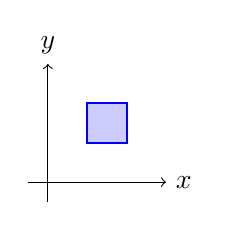
\begin{tikzpicture}[scale=0.5]
            \draw[->] (-0.5,0) -- (3,0) node[right] {$x$};
            \draw[->] (0,-0.5) -- (0,3) node[above] {$y$};
            \fill[blue!20] (1,1) rectangle (2,2);
            \draw[thick, blue] (1,1) rectangle (2,2);
        \end{tikzpicture}
        \caption{Item 39}
    \end{subfigure}\hfill
    \begin{subfigure}[b]{0.3\linewidth}
        \centering
        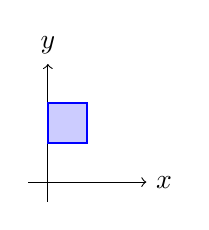
\begin{tikzpicture}[scale=0.5]
            \draw[->] (-0.5,0) -- (2.5,0) node[right] {$x$};
            \draw[->] (0,-0.5) -- (0,3) node[above] {$y$};
            \fill[blue!20] (0,1) rectangle (1,2);
            \draw[thick, blue] (0,1) rectangle (1,2);
        \end{tikzpicture}
        \caption{Item 40}
    \end{subfigure}\hfill
    \begin{subfigure}[b]{0.3\linewidth}
        \centering
        \begin{tikzpicture}[scale=0.5]
            \draw[->] (-2,0) -- (2,0) node[right] {$x$};
            \draw[->] (0,-0.5) -- (0,2) node[above] {$y$};
            \draw[very thick, blue] (-1,1) -- (1,1);
            \filldraw[blue] (-1,1) circle (2pt) (1,1) circle (2pt);
        \end{tikzpicture}
        \caption{Item 41}
    \end{subfigure}

    \vspace{0.5cm}

    \begin{subfigure}[b]{0.3\linewidth}
        \centering
        \begin{tikzpicture}[scale=0.5]
            \draw[->] (-0.5,0) -- (3,0) node[right] {$x$};
            \draw[->] (0,-0.5) -- (0,2) node[above] {$y$};
            \draw[very thick, blue] (2,0) -- (2,1);
            \filldraw[blue] (2,0) circle (2pt) (2,1) circle (2pt);
        \end{tikzpicture}
        \caption{Item 42}
    \end{subfigure}\hfill
    \begin{subfigure}[b]{0.3\linewidth}
        \centering
        \begin{tikzpicture}[scale=0.5]
            \draw[->] (-3,0) -- (3,0) node[right] {$x$};
            \draw[->] (0,-0.5) -- (0,2) node[above] {$y$};
            \draw[very thick, blue] (-2,0) -- (-2,1);
            \draw[very thick, blue] (2,0) -- (2,1);
            \filldraw[blue] (-2,0) circle (2pt) (-2,1) circle (2pt) (2,0) circle (2pt) (2,1) circle (2pt);
        \end{tikzpicture}
        \caption{Item 43}
    \end{subfigure}\hfill
    \begin{subfigure}[b]{0.3\linewidth}
        \centering
        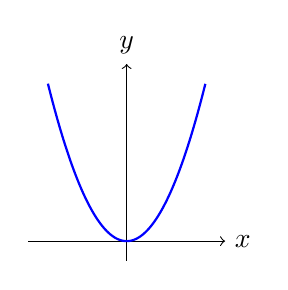
\begin{tikzpicture}[scale=0.5]
            \draw[->] (-2.5,0) -- (2.5,0) node[right] {$x$};
            \draw[->] (0,-0.5) -- (0,4.5) node[above] {$y$};
            \draw[thick, blue, domain=-2:2, samples=100] plot (\x, {\x*\x});
        \end{tikzpicture}
        \caption{Item 44}
    \end{subfigure}

    \vspace{0.5cm}

    \begin{subfigure}[b]{0.3\linewidth}
        \centering
        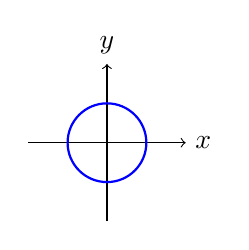
\begin{tikzpicture}[scale=0.5]
            \draw[->] (-2,0) -- (2,0) node[right] {$x$};
            \draw[->] (0,-2) -- (0,2) node[above] {$y$};
            \draw[thick, blue] (0,0) circle (1);
        \end{tikzpicture}
        \caption{Item 45}
    \end{subfigure}
    \caption{Geometric Representations 39--45}\label{fig:geom_part1}
\end{figure}
% --- SECOND PAGE: Items 46 to 52 ---
\begin{figure}[htbp]
    \ContinuedFloat% Keeps the figure numbering the same
    \centering
    \begin{subfigure}[b]{0.3\linewidth}
        \centering
        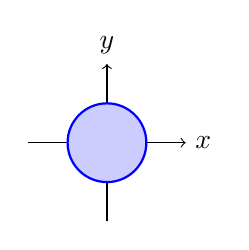
\begin{tikzpicture}[scale=0.5]
            \draw[->] (-2,0) -- (2,0) node[right] {$x$};
            \draw[->] (0,-2) -- (0,2) node[above] {$y$};
            \filldraw[fill=blue!20, draw=blue, thick] (0,0) circle (1);
        \end{tikzpicture}
        \caption{Item 46}
    \end{subfigure}\hfill
    \begin{subfigure}[b]{0.3\linewidth}
        \centering
        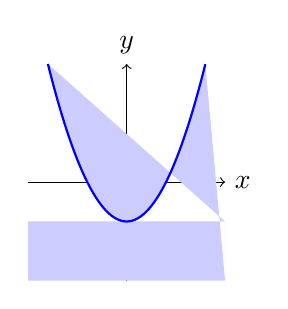
\begin{tikzpicture}[scale=0.5]
            \draw[->] (-2.5,0) -- (2.5,0) node[right] {$x$};
            \draw[->] (0,-2.5) -- (0,3) node[above] {$y$};
            \begin{scope}
                \clip (-2.5,-2.5) rectangle (2.5,3);
                \fill[blue!20] (-2.5,-2.5) rectangle (2.5,-1) -- plot[domain=-2:2, samples=100] (\x, {\x*\x - 1}) -- (2.5,-2.5);
                \draw[thick, blue, domain=-2:2, samples=100] plot (\x, {\x*\x - 1});
            \end{scope}
        \end{tikzpicture}
        \caption{Item 47}
    \end{subfigure}\hfill
    \begin{subfigure}[b]{0.3\linewidth}
        \centering
        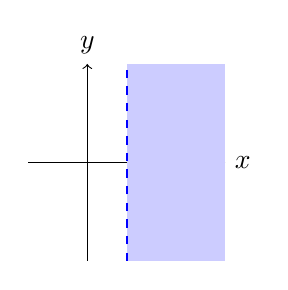
\begin{tikzpicture}[scale=0.5]
            \draw[->] (-1.5,0) -- (3.5,0) node[right] {$x$};
            \draw[->] (0,-2.5) -- (0,2.5) node[above] {$y$};
            \fill[blue!20] (1,-2.5) rectangle (3.5,2.5);
            \draw[dashed, thick, blue] (1,-2.5) -- (1,2.5);
        \end{tikzpicture}
        \caption{Item 48}
    \end{subfigure}

    \vspace{0.5cm}

    \begin{subfigure}[b]{0.3\linewidth}
        \centering
        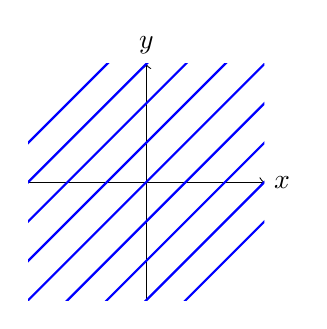
\begin{tikzpicture}[scale=0.5]
            \draw[->] (-3,0) -- (3,0) node[right] {$x$};
            \draw[->] (0,-3) -- (0,3) node[above] {$y$};
            \begin{scope}
                \clip (-3,-3) rectangle (3,3);
                \foreach \k in {-4,-3,...,4} {
                    \draw[thick, blue, domain=-4:4] plot (\x, {\x + \k});
                }
            \end{scope}
        \end{tikzpicture}
        \caption{Item 49}
    \end{subfigure}\hfill
    \begin{subfigure}[b]{0.3\linewidth}
        \centering
        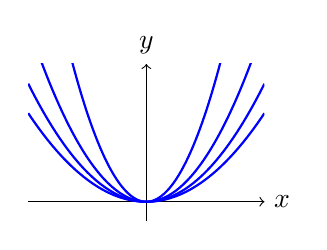
\begin{tikzpicture}[scale=0.5]
            \draw[->] (-3,0) -- (3,0) node[right] {$x$};
            \draw[->] (0,-0.5) -- (0,3.5) node[above] {$y$};
            \begin{scope}
                \clip (-3,-0.5) rectangle (3,3.5);
                \foreach \k in {1,2,3,4} {
                    \draw[thick, blue, domain=-3:3, samples=100] plot (\x, {(\x*\x)/\k});
                }
            \end{scope}
        \end{tikzpicture}
        \caption{Item 50}
    \end{subfigure}\hfill
    \begin{subfigure}[b]{0.3\linewidth}
        \centering
        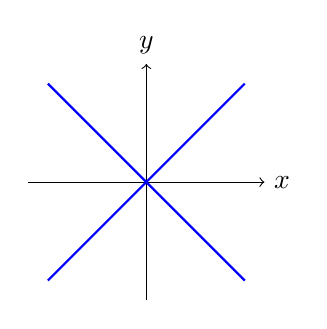
\begin{tikzpicture}[scale=0.5]
            \draw[->] (-3,0) -- (3,0) node[right] {$x$};
            \draw[->] (0,-3) -- (0,3) node[above] {$y$};
            \draw[thick, blue] (-2.5,-2.5) -- (2.5,2.5);
            \draw[thick, blue] (-2.5,2.5) -- (2.5,-2.5);
        \end{tikzpicture}
        \caption{Item 51}
    \end{subfigure}

    \vspace{0.5cm}

    \begin{subfigure}[b]{0.3\linewidth}
        \centering
        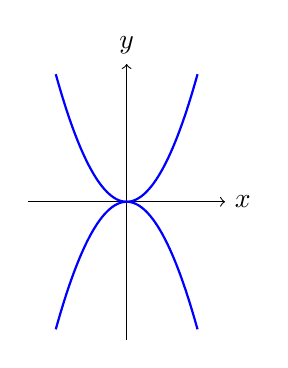
\begin{tikzpicture}[scale=0.5]
            \draw[->] (-2.5,0) -- (2.5,0) node[right] {$x$};
            \draw[->] (0,-3.5) -- (0,3.5) node[above] {$y$};
            \draw[thick, blue, domain=-1.8:1.8, samples=100] plot (\x, {\x*\x});
            \draw[thick, blue, domain=-1.8:1.8, samples=100] plot (\x, {-\x*\x});
        \end{tikzpicture}
        \caption{Item 52}
    \end{subfigure}

    \caption{Geometric Representations 46--52 (Continued)}\label{fig:geom_part2}
\end{figure}
\end{solution}

\section{Solutions to Exercises from Section 2}
\begin{solution}\label{sol:2.1}\ref{ex:2.1}
$$
\begin{aligned}
    &(a) A\times B =\{ (1,a),(1,c),(2,a),(2,c),(3,a),(3,c),(4,a),(4,c) \}\\\\
    &(b) B\times A =\{ (a,1),(c,1),(a,2),(c,2),(a,3),(c,3),(a,4),(c,4) \}\\\\
    &(c) A\times A =A^2= \{ (1,1),(1,2),(1,3),(1,4),(2,1),(2,2),(2,3),\\\\
    &(2,4),(3,1),(3,2),(3,3),(3,4),(4,1),(4,2),(4,3),(4,4) \}\\
    &(d) B\times B = B^2 = \{ (a,a),(a,c), (c,a),(c,c) \}\\\\
    &(e) \varnothing\times B= \{ (a,b):a\in\varnothing,b\in B \}= \varnothing\\\\
    &(f) (A\times B)\times B = \{ (1,a),(1,c),(2,a),(2,c),(3,a),(3,c),(4,a),(4,c) \}\times
    \{ a,c \}=\\
    &\{ ((1,a),a),((1,c),a), ((2,a),a),\\
    &((2,c),a), ((3,a),a),((3,c),a),\\
    &((4,a),a),((4,c),a), ((1,a),c),\\ 
    &((1,c),c),((2,a),c),((2,c),c),\\
    &((3,a),c),((3,c),c),((4,a),c),((4,c),c) \}\\\\
    &(g) A\times (B\times B) = \{ 1,2,3,4 \}\times \{ (a,a),(a,c),(c,a),(c,c) \}=\\
    &\{ (1,(a,a)),(1,(a,c)),(1,(c,a)),(1,(c,c)),\\
    &(2,(a,a)),(2,(a,c)),(2,(c,a)),(2,(c,c))\},\\
    &(3,(a,a)), (3,(a,c)), (3,(c,a)),(3,(c,c)),\\
    &(4,(a,a)),(4,(a,c)),(4,(c,a)),(4,(c,c))\\\\
    &(h) B^3=\{ (a,a,a),(a,a,c),(a,c,a), (a,c,c), (c,a,a),(c,a,c),(c,c,a),(c,c,c) \} = |2^3| = 8
\end{aligned}
$$
This ends Part I of~\ref{ex:2.1}. Now, for part II.\@
$$
\begin{aligned}
    &(a) A\times B= \{ (\pi,0),(\pi,1),(e,0),(e,1),(0,0),(0,1) \}\\\\
    &(b) B\times A= \{ (0,\pi),(1,\pi),(0,e),(1,e),(0,0),(1,0) \}\\\\
    &(c) A^2= \{ (\pi,\pi), (\pi,e),(\pi,0)\\
    &(e,\pi),(e,e),(e,0)\\
    &(0,\pi),(0,e),(0,0) \}\\\\
    &(d) B^2= \{ (0,0),(0,1),(1,0),(1,1) \}\\\\
    &(e) A\times\varnothing=\varnothing\\\\
    &(f) (A\times B)\times B= \{ (\pi,0),(\pi,1),(e,0),(e,1),(0,0),(0,1) \}\times \{ 0,1 \}\\
    &\{  ((\pi,0),0), ((\pi,0),1), ((\pi,1),0), \\
    &((\pi,1),1,), ((e,0),0),((e,0),1),\\
    &((e,1),0),((e,1),1), ((0,0),0),\\
    &((0,0),1), ((0,1),0),((0,1),1)\}\\\\
    &(g) A\times (B\times B)= \{ \pi,e,0 \}\times \{ (0,0),(0,1),(1,0),(1,1) \}\\
    &\{ (\pi,(0,0)),(\pi,(0,1)),(\pi,(1,0)),(\pi,(1,1)),\\
    &(e,(0,0)),(e,(0,1)),(e,(1,0)),(e,(1,1))\\
    &(0,(0,0)),(0,(0,1)),(0,(1,0)),(0,(1,1)) \}\\\\
    &(h) A\times B\times B=\{ (\pi, 0,0),(\pi,0,1),(\pi,1,0),\\
    &(\pi,1,1),(e,0,0),(e,0,1),\\
    &(e,1,0),(e,1,1),(0,0,0),\\
    &(0,0,1),(0,1,0),(0,1,1) \}
\end{aligned}
$$
This concludes part II.\@ Lastly, part III.\@
$$
\begin{aligned}
    &(3)~ \{ x\in\R:x^2=2 \}\times \{ a,c,e \}=\\
    &\{ -\sqrt 2, \sqrt 2 \}\times \{ a,c,e \}=\\
    &\{ (-\sqrt 2, a),(-\sqrt 2, c),(-\sqrt 2, e),\\
    &(\sqrt 2, a),(\sqrt 2,c),(\sqrt 2, e)\}\\\\
    &(4)~ \{ n\in\Z:2<n<5 \}\times \{ n\in\Z:\lvert n \rvert=5 \}=\\
    &\{ 3,4 \}\times \{ -5,5 \}=\{ (3,-5),(3,5),(4,-5),(4,5) \}\\\\
    &(5)~\{ x\in\R:x^2=2 \}\times \{ x\in\R:\lvert x \rvert=2 \}=\\
    &\{ -\sqrt2,\sqrt 2 \}\times \{ -2,2 \}= \{ (-\sqrt 2,-2),(-\sqrt 2,2),(\sqrt 2,-2),(\sqrt 2,2) \}\\\\
    &(6)~\{ x\in\R:x^2=x \}\times \{ x\in\N:x^2=x \}=\\
    &\{ -1,0,1 \}\times \{ 0,1 \}=\\
    &\{ (-1,0),(-1,1),(0,0),(0,1),(1,0),(1,1) \}\\\\
    &(7)~\{ \varnothing \}\times \{ 0,\varnothing \}\times \{ 0,1 \}=\\
    &\{ (\varnothing ,0,0),(\varnothing,\varnothing, 0),( \varnothing ,0,1),( \varnothing , \varnothing, 1) \}\\\\
    &(8)~\{ 0,1 \}{^4}=\{(0,0,0,0),(0,0,0,1),(0,0,1,0),(0,1,0,0),\\
    &(1,0,0,0),(0,0,1,1),(0,1,0,1),(1,0,0,1),\\
    &(0,1,1,0),(1,1,0,0),(1,1,1,0),(1,1,1,1),\\
    &(0,1,1,1),(1,0,1,0), (1,0,1,1),(1,1,0,1)\}.
\end{aligned}
$$


\end{solution}
\begin{solution}\label{sol:2.2}\ref{ex:2.2}
    As in the previous exercise where we sketched out the sets on the $xy$-plane, we will first solve them/explain them and then go on to sketch them.
    $$
    \begin{aligned}
        &(9) \{ 1,2,3 \}\times \{ -1,0,1 \}=\\
        &\{ (1,-1),(1,0),(1,1),\\
        &(2,-1),(2,0),(2,1),\\
        &(3,-1),(3,0),(3,1) \}\\\\
        &(10) \{ -1,0,1 \}\times \{ 1,2,3 \}=\\
        &\{ (-1,1),(-1,2),(-1,3),\\
        & (0,1),(0,2),(0,3),\\
        & (1,1),(1,2),(1,3) \}\\\\
        &(11) [0,1]\times [0,1] \text{ these would be all the paired points in that interval starting from }\\
        &x=0,y=1\\\\
        &(12) [-1,1]\times [1,2] \text{ these would be all the paired points in that interval starting from }\\
        &x=-1,y=1 \text{ and filling the space up to } x=1,y=2\\\\
        &(13) \{ 1,1.5,2 \}\times [1,2] \text{ similarly to the cases above, those will become more obvious when we sketch them out}\\\\
        &(14) [1,2]\times \{ 1,1.5,2 \}, \text{ ditto.}\\\\
        &(15) \{ 1 \}\times [0,1]\\\\
        &(16) [0,1]\times \{ 1 \}\\\\
        &(17) \N\times\Z,\text{ here, we take the natural numbers as our first coordinate and the integers as our second.}\\\\
        &(18) \Z^2,\text{ here we have the whole } xy \text{-plane with whole positive and negative integers.}\\\\
        &(19) [0,1]{^2}\\\\
        &(20) \{ (x,y)\in\R^2:x^2+y^2\le 1 \}\times [0,1].
    \end{aligned}
    $$
    Now, we will show them plotted on the $xy$-plane. 

    % --- FIRST PAGE: Items 9 to 14 ---
\begin{figure}[htbp]
    \centering
    % Item 9
    \begin{subfigure}[b]{0.3\linewidth}
        \centering
        \begin{tikzpicture}[scale=0.6]
            \draw[->] (-0.5,0) -- (3.8,0) node[right] {$x$};
            \draw[->] (0,-1.8) -- (0,1.8) node[above] {$y$};
            \foreach \x in {1,2,3} {
                \foreach \y in {-1,0,1} {
                    \fill[blue] (\x,\y) circle (2.5pt);
                }
            }
        \end{tikzpicture}
        \caption{Item (9)}
    \end{subfigure}\hfill
    % Item 10
    \begin{subfigure}[b]{0.3\linewidth}
        \centering
        \begin{tikzpicture}[scale=0.6]
            \draw[->] (-1.8,0) -- (1.8,0) node[right] {$x$};
            \draw[->] (0,-0.5) -- (0,3.8) node[above] {$y$};
            \foreach \x in {-1,0,1} {
                \foreach \y in {1,2,3} {
                    \fill[blue] (\x,\y) circle (2.5pt);
                }
            }
        \end{tikzpicture}
        \caption{Item (10)}
    \end{subfigure}\hfill
    % Item 11
    \begin{subfigure}[b]{0.3\linewidth}
        \centering
        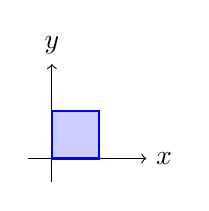
\begin{tikzpicture}[scale=0.6]
            \draw[->] (-0.5,0) -- (2,0) node[right] {$x$};
            \draw[->] (0,-0.5) -- (0,2) node[above] {$y$};
            \fill[blue!20] (0,0) rectangle (1,1);
            \draw[thick, blue] (0,0) rectangle (1,1);
        \end{tikzpicture}
        \caption{Item (11)}
    \end{subfigure}

    \vspace{0.6cm}

    % Item 12
    \begin{subfigure}[b]{0.3\linewidth}
        \centering
        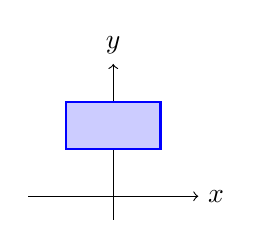
\begin{tikzpicture}[scale=0.6]
            \draw[->] (-1.8,0) -- (1.8,0) node[right] {$x$};
            \draw[->] (0,-0.5) -- (0,2.8) node[above] {$y$};
            \fill[blue!20] (-1,1) rectangle (1,2);
            \draw[thick, blue] (-1,1) rectangle (1,2);
        \end{tikzpicture}
        \caption{Item (12)}
    \end{subfigure}\hfill
    % Item 13
    \begin{subfigure}[b]{0.3\linewidth}
        \centering
        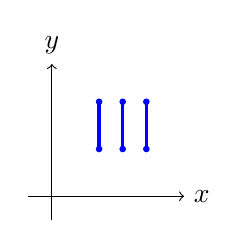
\begin{tikzpicture}[scale=0.6]
            \draw[->] (-0.5,0) -- (2.8,0) node[right] {$x$};
            \draw[->] (0,-0.5) -- (0,2.8) node[above] {$y$};
            \foreach \x in {1,1.5,2} {
                \draw[very thick, blue] (\x,1) -- (\x,2);
                \fill[blue] (\x,1) circle (2pt) (\x,2) circle (2pt);
            }
        \end{tikzpicture}
        \caption{Item (13)}
    \end{subfigure}\hfill
    % Item 14
    \begin{subfigure}[b]{0.3\linewidth}
        \centering
        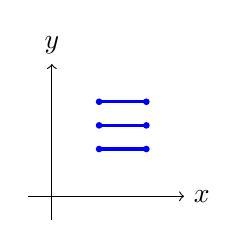
\begin{tikzpicture}[scale=0.6]
            \draw[->] (-0.5,0) -- (2.8,0) node[right] {$x$};
            \draw[->] (0,-0.5) -- (0,2.8) node[above] {$y$};
            \foreach \y in {1,1.5,2} {
                \draw[very thick, blue] (1,\y) -- (2,\y);
                \fill[blue] (1,\y) circle (2pt) (2,\y) circle (2pt);
            }
        \end{tikzpicture}
        \caption{Item (14)}
    \end{subfigure}

    \caption{Plots for Cartesian Products (Items 9--14)}\label{fig:cartesian_1}
\end{figure}

% --- SECOND PAGE: Items 15 to 20 ---
\begin{figure}[htbp]
    \ContinuedFloat%
    \centering
    % Item 15
    \begin{subfigure}[b]{0.3\linewidth}
        \centering
        \begin{tikzpicture}[scale=0.6]
            \draw[->] (-0.5,0) -- (2.2,0) node[right] {$x$};
            \draw[->] (0,-0.5) -- (0,2) node[above] {$y$};
            \draw[very thick, blue] (1,0) -- (1,1);
            \fill[blue] (1,0) circle (2pt) (1,1) circle (2pt);
        \end{tikzpicture}
        \caption{Item (15)}
    \end{subfigure}\hfill
    % Item 16
    \begin{subfigure}[b]{0.3\linewidth}
        \centering
        \begin{tikzpicture}[scale=0.6]
            \draw[->] (-0.5,0) -- (2,0) node[right] {$x$};
            \draw[->] (0,-0.5) -- (0,2) node[above] {$y$};
            \draw[very thick, blue] (0,1) -- (1,1);
            \fill[blue] (0,1) circle (2pt) (1,1) circle (2pt);
        \end{tikzpicture}
        \caption{Item (16)}
    \end{subfigure}\hfill
    % Item 17
    \begin{subfigure}[b]{0.3\linewidth}
        \centering
        \begin{tikzpicture}[scale=0.6]
            \draw[->] (-0.5,0) -- (3.2,0) node[right] {$x$};
            \draw[->] (0,-2.2) -- (0,2.2) node[above] {$y$};
            \foreach \x in {1,2,3} {
                \foreach \y in {-2,-1,0,1,2} {
                    \fill[blue] (\x,\y) circle (2pt);
                }
            }
            \node[blue] at (3.1, 0) {$\dots$};
            \node[blue] at (2, 2.1) {$\vdots$};
            \node[blue] at (2, -2.1) {$\vdots$};
        \end{tikzpicture}
        \caption{Item (17) $\mathbb{N} \times \mathbb{Z}$}
    \end{subfigure}

    \vspace{0.6cm}

    % Item 18
    \begin{subfigure}[b]{0.3\linewidth}
        \centering
        \begin{tikzpicture}[scale=0.6]
            \draw[->] (-2.2,0) -- (2.2,0) node[right] {$x$};
            \draw[->] (0,-2.2) -- (0,2.2) node[above] {$y$};
            \foreach \x in {-2,-1,0,1,2} {
                \foreach \y in {-2,-1,0,1,2} {
                    \fill[blue] (\x,\y) circle (2pt);
                }
            }
            \node[blue] at (2.1, 0) {$\dots$};
            \node[blue] at (-2.1, 0) {$\dots$};
            \node[blue] at (0, 2.1) {$\vdots$};
            \node[blue] at (0, -2.1) {$\vdots$};
        \end{tikzpicture}
        \caption{Item (18) $\mathbb{Z}^2$}
    \end{subfigure}\hfill
    % Item 19
    \begin{subfigure}[b]{0.3\linewidth}
        \centering
        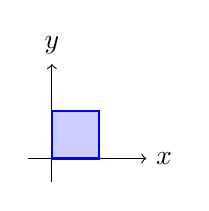
\begin{tikzpicture}[scale=0.6]
            \draw[->] (-0.5,0) -- (2,0) node[right] {$x$};
            \draw[->] (0,-0.5) -- (0,2) node[above] {$y$};
            \fill[blue!20] (0,0) rectangle (1,1);
            \draw[thick, blue] (0,0) rectangle (1,1);
        \end{tikzpicture}
        \caption{Item (19) $[0,1]{^2}$}
    \end{subfigure}\hfill
    % Item 20
    \begin{subfigure}[b]{0.3\linewidth}
        \centering
        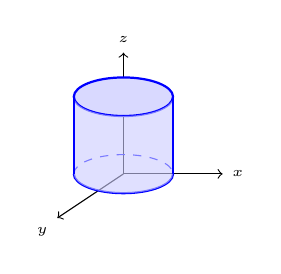
\begin{tikzpicture}[scale=0.7]
            % 3D Axes
            \draw[->] (0,0) -- (1.8,0) node[right] {\tiny $x$};
            \draw[->] (0,0) -- (0,2.2) node[above] {\tiny $z$};
            \draw[->] (0,0) -- (-1.2,-0.8) node[below left] {\tiny $y$};
            
            % Cylinder Body (Solid Disk x [0,1])
            \filldraw[fill=blue!15, draw=blue, thick] (0,1.4) ellipse (0.9cm and 0.35cm);
            \draw[thick, blue] (-0.9,0) arc (180:360:0.9cm and 0.35cm);
            \draw[dashed, blue] (-0.9,0) arc (180:0:0.9cm and 0.35cm);
            \fill[blue!20, opacity=0.6] (-0.9,0) arc (180:360:0.9cm and 0.35cm) -- (0.9,1.4) arc (0:-180:0.9cm and 0.35cm) -- cycle;
            \draw[thick, blue] (-0.9,0) -- (-0.9,1.4);
            \draw[thick, blue] (0.9,0) -- (0.9,1.4);
        \end{tikzpicture}
        \caption{Item (20) Disk $\times [0,1]$}
    \end{subfigure}

    \caption{Plots for Cartesian Products (Items 15--20, Continued)}\label{fig:cartesian_2}
\end{figure}
\end{solution}

\section*{Solutions to Exercises from Section 3}
\begin{solution}\label{sol:3.1}\ref{ex:3.1}
    
    $$
    \begin{aligned}
        &(1)~ \{ 1,2,3,4 \}=\\
        &\varnothing, \{ 1 \},\{ 2 \},\{ 3 \},\{ 4 \},\\
        &\{ 1,2 \},\{ 1,3 \},\{ 1,4 \},\{ 2,3 \},\\
        &\{ 2,4 \}, \{ 3,4 \},\{ 1,2,3 \},\{ 1,2,4 \},\\
        &\{ 1,3,4 \}, \{ 2,3,4 \}, \{ 1,2,3,4 \}\\\\
        &(2)~\{ 1,2,\varnothing \}=\\
        &\varnothing, \{ 1 \},\{ 2\},\\
        &\{ \varnothing \}, \{ 1,2 \},\{ 1,\varnothing \},\\
        &\{ 2,\varnothing \}, \{ 1,2,\varnothing \}\\\\
        &(3)~ \{ \{ \R \} \}=\varnothing, \{ \R \}\\\\
        &(4)~\varnothing = \varnothing\\\\
        &(5)~\{ \varnothing \}=\varnothing, \{ \varnothing \}\\\\
        &(6)~\{ \R,\Q,\N \}=\\
        &\varnothing, \{ \R \},\{ N \},\{ \Q \},\\
        &\{ \R,\N \},\{ \R,\Q \}, \{ \N,\Q \},\{ \R,\N,\Q \}\\\\
        &(7)~\{ \R,\{ \N,\Q \} \}=\\
        &\varnothing, \{ \R \},\{\{ \N,\Q \}\}, \{ \R,\{ \N,\Q \} \}\\\\
        &(8)~\{ \{ 0,1 \},\{ 0,1,\{ 2 \} \},\{ 0 \} \}=\\
        &\varnothing, \{\{ 0,1 \}\}, \{\{ 0,1,\{ 2 \} \}\},\{\{ 0 \}\},\\
        &\{ \{ 0,1 \},\{ 0,1,\{ 2 \} \} \}, \{ \{ 0,1 \}, \{ 0 \} \},\\
        &\{ \{ 0,1,\{ 2 \} \},\{ 0 \} \}, \{ \{ 0,1 \},\{ 0,1,\{ 2 \} \},\{ 0 \} \}.
    \end{aligned}
    $$
\end{solution}

\begin{solution}\label{sol:3.2}\ref{ex:3.2}
    $$
    \begin{aligned}
    &(1)~\{ X:X\subseteq \{ 3,2,a \}\text{ and } \lvert X \rvert=2 \}=\{ \{ 3,2 \},\{ 3,a \},\{ 2,a \} \}\\\\
    &(2)~\{ X\subseteq\N:\lvert X \rvert\le 1 \}=\{ \varnothing \}\cup \{ \{ n \}:n\in\N \}\\\\
    &(3)~\{ X:X\subseteq \{ 3,2,a \}\text{ and }\lvert X \rvert=4 \}=\varnothing\\\\
    &(4)~\{ X:X\subseteq \{ 3,2,a \}\text{ and }\lvert X \rvert=1 \}=\{ \{ 3 \},\{ 2 \},\{ a \} \}\\\\
    \end{aligned}
    $$ 
   \end{solution}

\begin{solution}\label{sol:3.3}\ref{ex:3.3}
   
   $$
   (1)~\R^3\subseteq\R^3
   $$

   $(1)$ is true, for the fact that every set is a subset of itself. 
   
   $$
   (2)~\R^2\subseteq\R^3
   $$
   $(2)$ is tricky, strictly speaking it is false. However, if you have any experience with Linear Algebra you might consider it true. In Linear Algebra we abuse the notation and say that $\R^3$ is an extension of $\R^2$, addiing the third dimension to a two dimensional plane. In set theory however, we are a bit more strict. The above is false, since 
   $$
   \R^2=\R\times\R=\{ (x,y):x\in \R\land y\in\R \},
   $$
   And 
   $$
   \R^3=\R\times\R\times\R=\{ (x,y,z):x\in\R\land y\in\R \land z\in\R \}.
   $$
   So, the first \emph{object} takes in pairs, and the second object takes in triples. 

   $$
   (3)~\{ (x,y)\in\R^2:x-1=0 \}\subseteq \{ (x,y)\in\R^2:x^2-x=0 \}.
   $$
   Consider a small example here, the set contains pairs $(x,y)$, the first element of the pair has to be $1$, so $\{ (1,y):y\in\R \}$. In the second set we have $x^2-x=0$, solving this gives us $x=0,\lor x=1$, so we have the pairs $\{ (0,y),(1,y):y\in\R \}$. Then it follows that the example is true. 
   $$
   (4)~\{ (x,y)\in\R^2:x^2-x=0 \}\subseteq \{ (x,y)\in\R^2:x-1=0 \}.
   $$
   This example is false, in the LHS, we can have $0^2-0=0$, whereas in the RHS we cannot, unless $x=1$.  
\end{solution}
\section{Solutions to Exercises from Section 4}
\begin{solution}\label{sol:4.1}\ref{ex:4.1}
    I will also show the cardinality of the powerset since I think it helps with counting all its subsets.
    $$
    \begin{aligned}
        &(1)~\powerset(\{\{ a,b \},\{ c \}\}) = \{ \varnothing,\{ \{ a,b \} \},\{ \{ c \} \},\{ \{ a,b \},\{ c \} \} \}\quad  \lvert \powerset(\{ \{ a,b \},\{ c \} \}) \rvert=2^2=4 \text{ elements}\\\\
        &(2)~\powerset(\{ 1,2,3,4 \})= \{ \varnothing,\{ 1 \},\{ 2 \},\{ 3 \},\{ 4 \},\\
        &\{ 1,2 \},\{ 1,3 \},\{ 1,4 \},\{ 2,3 \},\{ 2,4 \},\\
        &\{ 3,4 \},\{ 1,2,3 \},\{ 1,2,4 \},\{ 1,3,4 \},\{ 2,3,4 \},\{ 1,2,3,4 \} \}=2^4=16 \text{ elements}. \\\\
        &(3)~\powerset(\{ \{ \varnothing \},5 \})= \{ \varnothing,\{ \{ \varnothing \} \},\{ 5 \}, \{ \{ \varnothing \},5 \} \}=2^2=4 \text{ elements}.\\\\
        &(4)~ \powerset(\{ \R,\Q \})= \{ \varnothing, \{ \R \},\{ \Q \},\{ \R,\Q \} \}=2^2=4 \text{ elements}. \\\\
        &(5)~\powerset(\powerset(\{ 2 \}))=\powerset(\{ \varnothing, \{ 2 \} \})=\\
        &\{ \varnothing,\{ \varnothing \}, \{ \{ 2 \} \}, \{ \varnothing, \{ 2 \} \} \}=2^2=4 \text{ elements.}\\\\
        &(6)~\powerset(\{ 1,2 \})\times\powerset(\{ 3 \})=\\
        &\{ \varnothing,\{ 1 \},\{ 2 \},\{ 1,2 \} \}\times \{ \varnothing, \{ 3 \} \}=\\
        & \{ (\varnothing, \varnothing), (\varnothing, \{ 3 \}), (\{ 1 \},\varnothing), (\{ 1 \},\{ 3 \}),\\
        & (\{ 2 \},\varnothing),(\{ 2 \},\{ 3 \}), (\{ 1,2 \},\varnothing),(\{ 1,2 \},\{ 3 \}) \}\\\\
        &(7)~\powerset(\{ a,b \})\times\powerset(\{ 0,1 \})=\\
        & \{ \varnothing,\{ a \},\{ b \},\{ a,b \} \}\times \{ \varnothing,\{ 0 \},\{ 1 \},\{ 0,1 \} \}=\\
        & \{ (\varnothing,\varnothing), (\varnothing, \{ 0 \}),(\varnothing, \{ 1 \}),(\varnothing, \{ 0,1 \}),\\
        &(\{ a \},\varnothing),(\{ a \},\{ 0 \}),(\{ a \},\{ 1 \}),(\{ a \},\{ 0,1 \}),\\
        &(\{ b \},\varnothing),(\{ b \},\{ 0 \}),(\{ b \},\{ 1 \}), (\{ b \},\{ 0,1 \}),\\
        &(\{ a,b \},\varnothing),(\{ a,b \},\{ 0 \}),(\{ a,b \},\{ 1 \}),(\{ a,b \},\{ 0,1 \}) \}\\\\
        &(8)~\powerset(\{ 1,2 \}\times \{ 3 \})= \powerset(\{ (1,3),(2,3) \})=\\
        & \{ \varnothing, \{ (1,3) \},\{ (2,3) \},\{ (1,3),(2,3) \} \}\\\\
        &(9)~\powerset(\{ a,b \}\times \{ 0 \})=\powerset(\{ (a,0),(b,0) \})=\\
        &\{ \varnothing,\{ (a,0) \},\{ (b,0) \},\{ (a,0),(b,0) \} \}
    \end{aligned}
    $$
    We will do the last three examples separately, since there is a bit more to consider. Let's start with $(10)$:
    $$
    (10)~\{ X\in\powerset(\{ 1,2,3 \}): \lvert X \rvert\le 1 \}
    $$
    Notice that we are looking for a \emph{member} $X$, that has size no bigger than $1$. So, let's count the powerset and then see which sets qualify. 
    $$
    \begin{aligned}
        &\powerset(\{ 1,2,3 \})= \{ \varnothing, \{ 1 \},\{ 2 \},\{ 3 \},\\
        &\{ 1,2 \},\{ 1,3 \},\{ 2,3 \},\{ 1,2,3 \} \}=2^3=8 \text{elements}
    \end{aligned}
    $$
    Now, for the condition $X\in\powerset(\{ 1,2,3 \})$. We have 
    $$
    \{\varnothing, \{ 1 \},\{ 2 \},\{ 3 \}\}.
    $$
These are all the singletons and the empty set. For $(11)$, we have 
$$
\{ \varnothing,\{ \varnothing \}, \{ \{ 1 \} \},\{ \{ 2 \} \},\{ \{ 3 \} \}, \{ \{ 1,2 \} \},\{ \{ 1,3 \} \},\{ \{ 2,3 \} \},\{ \{ 1,2,3 \} \} \}.
$$
This might seem strange, but these are all of cardinality at most than $1$. Notice that the subsets of the powerset are all enclosed in an extra pair of curly braces, so they are counted as having one element. Lastly, for $(12)$ the condition changes slightly, we need to find $X\in\powerset(\{ 1,2,3 \})$ such that $2\in X$. So, 
$$
\{\{ 2 \},\{ 1,2 \},\{ 2,3 \},\{ 1,2,3 \}\}.
$$    
\end{solution}

\begin{solution}\label{sol:4.2}\ref{ex:4.2}
    We let $\lvert A \rvert= m ,\lvert B \rvert= n$, then 
    $$
    \begin{aligned}
        &(1)~\lvert \powerset\powerset\powerset(A) \rvert=2^{2^{2^{m}}}\\\\
        &(2)~\lvert \powerset\powerset(A) \rvert=2^{2^{m}}\\\\
        &(3)~\lvert \powerset(A\times B) \rvert=2^{m\cdot n}\\\\
        &(4)~\lvert \powerset(A)\times \powerset(B) \rvert=2^{m}\cdot 2^{n}\\\\
        &(5)~\lvert \{ X\in\powerset(A):\lvert X \rvert\le 1 \} \rvert= m+1\\\\
        &(6)~\lvert \powerset(A\times\powerset(B)) \rvert=2^{m\cdot 2^{n}}\\\\
        &(7)~ \lvert \powerset\powerset\powerset(A\times\varnothing) \rvert=4\\\\
        &(8)~\lvert \{ X\subseteq\powerset(A):\lvert X \rvert\le 1 \} \rvert=2^{m}+1.
    \end{aligned}
    $$
    \emph{Some Further Comments:} For $(5)$ it is important to understand the following. We are looking at members of the powerset, as in the previous exercise, we saw that these would be all the singletons and the empty set. Since we have exactly $m$ singletons and we add the empty set to that, so we get $m+1$. 
    Since the product of any set with the empty set is empty, we have to calculate $\lvert \powerset\powerset\powerset(\varnothing) \rvert$. The idea in $(8)$ is the same as in the previous exercise. 
\end{solution}

\section{Solutions to Exercises from Section 5}
\begin{solution}\label{sol:5.1}\ref{ex:5.1}
    \begin{enumerate}
        \item $A\cup B=\{ 1,3,4,5,6,7,8,9 \}$
        \item $A\cap B=\{ 4,6 \}$
        \item $A-B=\{ 1,3,7,9 \}$
        \item $A-C=\{ 1,3,6,7,9 \}$
        \item $B-A=\{ 5,8 \}$
        \item $A\cap C=\{ 4 \}$
        \item $B\cap C=\{ 4,5,8 \}$
        \item $B\cup C=\{ 4,5,6,8 \}$
        \item $C-B=\varnothing$
    \end{enumerate}
\end{solution}

\begin{solution}\label{sol:5.2}\ref{ex:5.2}
    \begin{enumerate}
        \item $A\cup B=\{ 0,1,2,3,4,5,6,7,8 \}$
        \item $A\cap B=\varnothing$
        \item $A-B=A$ since $A\cap B=\varnothing$ (or in other words are disjoint)
        \item $A-C=\{ 0,6 \}$
        \item $B-A=B$ 
        \item $A\cap C=\{ 2,8,4 \}$
        \item $B\cap C=\varnothing$
        \item $B\cup C=\{ 1,2,3,4,5,7,8 \}$
        \item $C-B=C$
    \end{enumerate}
\end{solution}

\section*{Solutions to Exercises from Section 6}

\begin{solution}\label{sol:6.1}\ref{ex:6.1}
    \begin{enumerate}
        \item $A^{\complement}=\{ 0,2,5,8,10 \}$
        \item $B^{\complement}=\{ 0,1,2,3,7,9,10 \}$
        \item $A\cap A^{\complement}=\{ 0,2,5,8,10 \}\cap \{ 4,3,6,7,1,9 \}=\varnothing$
        \item $A\cup A^{\complement}=U$ by the same logic as the above example
        \item $A-A^{\complement}=\{ 0,2,5,8,10 \}-\{ 4,3,6,7,1,9 \}=\{ 0,2,5,8,10 \}=A$
        \item $A-B^{\complement}=\{ 4,6 \}$
        \item $A^{\complement}-B^{\complement}=\{ 5,8 \}$
        \item $A^{\complement}\cap B=\{ 5,8 \}$
        \item ${(A^{\complement}-B)}^{\complement}=\{ 1,3,4,5,6,7,9 \}$
    \end{enumerate}
\end{solution}

\begin{solution}\label{sol:6.2}\ref{ex:6.2}
    \begin{enumerate}
        \item $A^{\complement}=\{ 1,3,5,7 \}=B$
        \item $B^{\complement}=\{ 0,2,4,6,8 \}=A$
        \item $A\cap A^{\complement}=\varnothing$
        \item $A\cup A^{\complement}=U$
        \item $A-A^{\complement}=A$
        \item ${(A\cup B)}^{\complement}=\varnothing$
        \item $A^\complement\cap B^{\complement}=\varnothing$
        \item ${(A\cap B)}^{\complement}=U$
        \item $A^{\complement}\times B=\{ (1,1),(1,3),(1,5),\dots \}=B^{2}$
    \end{enumerate}
\end{solution}

\begin{solution}\label{sol:6.3}\ref{ex:6.3}
    You can find the solution for this exercise below. 
    \begin{figure}[htbp]
    \centering
    % Drawing 1: The set X
    \begin{subfigure}[b]{0.32\linewidth}
        \centering
        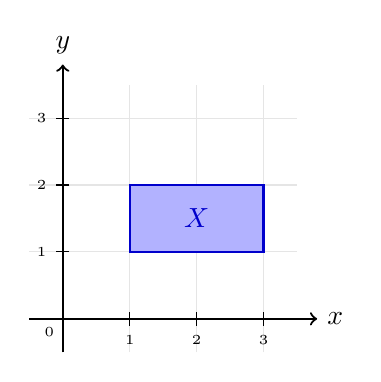
\begin{tikzpicture}[scale=0.85]
            % Grid & Axes
            \draw[gray!20, thin] (-0.5,-0.5) grid (3.5,3.5);
            \draw[->, thick] (-0.5,0) -- (3.8,0) node[right] {$x$};
            \draw[->, thick] (0,-0.5) -- (0,3.8) node[above] {$y$};
            
            % Ticks
            \foreach \x in {1,2,3} \draw (\x,0.1) -- (\x,-0.1) node[below] {\tiny $\x$};
            \foreach \y in {1,2,3} \draw (0.1,\y) -- (-0.1,\y) node[left] {\tiny $\y$};
            \node at (-0.2,-0.2) {\tiny $0$};

            % Set X: Shaded rectangle [1,3] x [1,2]
            \fill[blue!30] (1,1) rectangle (3,2);
            \draw[thick, blue!80!black] (1,1) rectangle (3,2);
            
            \node[blue!80!black] at (2,1.5) {$X$};
        \end{tikzpicture}
        \caption{The set $X = [1,3]\times[1,2]$}
    \end{subfigure}\hfill
    % Drawing 2: The set X^c
    \begin{subfigure}[b]{0.32\linewidth}
        \centering
        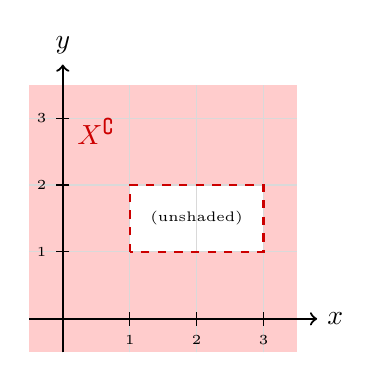
\begin{tikzpicture}[scale=0.85]
            % Outer shaded plane bounding box
            \fill[red!20] (-0.5,-0.5) rectangle (3.5,3.5);
            
            % Unshade the "hole" X
            \fill[white] (1,1) rectangle (3,2);
            
            % Grid & Axes
            \draw[gray!30, thin] (-0.5,-0.5) grid (3.5,3.5);
            \draw[->, thick] (-0.5,0) -- (3.8,0) node[right] {$x$};
            \draw[->, thick] (0,-0.5) -- (0,3.8) node[above] {$y$};
            
            % Ticks
            \foreach \x in {1,2,3} \draw (\x,0.1) -- (\x,-0.1) node[below] {\tiny $\x$};
            \foreach \y in {1,2,3} \draw (0.1,\y) -- (-0.1,\y) node[left] {\tiny $\y$};
            
            % Boundary of hole X
            \draw[thick, dashed, red!80!black] (1,1) rectangle (3,2);
            
            \node[red!80!black] at (0.5,2.8) {$X^{\complement}$};
            \node at (2,1.5) {\tiny (unshaded)};
        \end{tikzpicture}
        \caption{The complement $X^{\complement}$}
    \end{subfigure}\hfill
    % Drawing 3: X^c \cap ([0,2] \times [0,3])
    \begin{subfigure}[b]{0.32\linewidth}
        \centering
        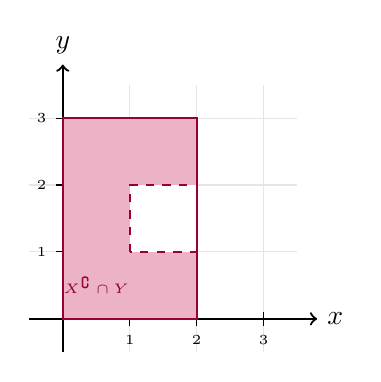
\begin{tikzpicture}[scale=0.85]
            % Grid & Axes
            \draw[gray!20, thin] (-0.5,-0.5) grid (3.5,3.5);
            \draw[->, thick] (-0.5,0) -- (3.8,0) node[right] {$x$};
            \draw[->, thick] (0,-0.5) -- (0,3.8) node[above] {$y$};
            
            % Ticks
            \foreach \x in {1,2,3} \draw (\x,0.1) -- (\x,-0.1) node[below] {\tiny $\x$};
            \foreach \y in {1,2,3} \draw (0.1,\y) -- (-0.1,\y) node[left] {\tiny $\y$};
            
            % Full region [0,2] x [0,3] shaded
            \fill[purple!30] (0,0) rectangle (2,3);
            % Hole where X overlaps: [1,2] x [1,2]
            \fill[white] (1,1) rectangle (2,2);
            
            % Outer boundary of [0,2] x [0,3]
            \draw[thick, purple!80!black] (0,0) rectangle (2,3);
            % Boundary of the removed hole
            \draw[thick, dashed, purple!80!black] (1,1) rectangle (2,2);
            
            \node[purple!80!black, font=\tiny] at (0.5,0.5) {$X^{\complement} \cap Y$};
        \end{tikzpicture}
        \caption{$X^{\complement}\cap([0,2]\times[0,3])$}
    \end{subfigure}

    \caption{Sketches of $X$, its complement $X^{\complement}$, and the restricted intersection.}\label{fig:ex_6_3}
\end{figure}
\end{solution}

\begin{solution}\label{sol:6.4}\ref{ex:6.4}
    Ditto.

    \begin{figure}[htbp]
    \centering
    % Drawing 1: The set X
    \begin{subfigure}[b]{0.32\linewidth}
        \centering
        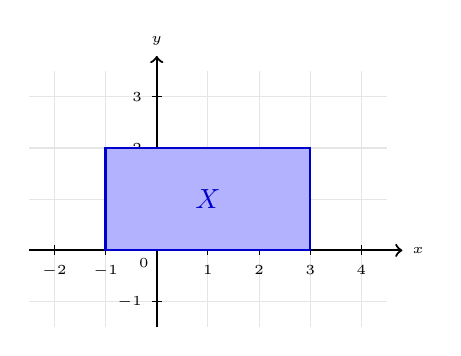
\begin{tikzpicture}[scale=0.65]
            % Grid & Axes
            \draw[gray!20, thin] (-2.5,-1.5) grid (4.5,3.5);
            \draw[->, thick] (-2.5,0) -- (4.8,0) node[right] {\tiny $x$};
            \draw[->, thick] (0,-1.5) -- (0,3.8) node[above] {\tiny $y$};
            
            % Ticks
            \foreach \x in {-2,-1,1,2,3,4} \draw (\x,0.1) -- (\x,-0.1) node[below] {\tiny $\x$};
            \foreach \y in {-1,1,2,3} \draw (0.1,\y) -- (-0.1,\y) node[left] {\tiny $\y$};
            \node at (-0.25,-0.25) {\tiny $0$};

            % Set X: Shaded rectangle [-1,3] x [0,2]
            \fill[blue!30] (-1,0) rectangle (3,2);
            \draw[thick, blue!80!black] (-1,0) rectangle (3,2);
            
            \node[blue!80!black] at (1,1) {$X$};
        \end{tikzpicture}
        \caption{The set $X$}
    \end{subfigure}\hfill
    % Drawing 2: The set X^c
    \begin{subfigure}[b]{0.32\linewidth}
        \centering
        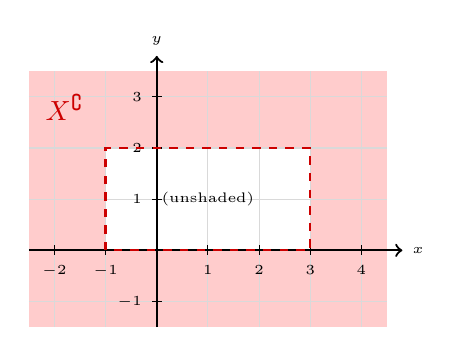
\begin{tikzpicture}[scale=0.65]
            % Outer shaded plane bounding box
            \fill[red!20] (-2.5,-1.5) rectangle (4.5,3.5);
            
            % Unshade the "hole" X
            \fill[white] (-1,0) rectangle (3,2);
            
            % Grid & Axes
            \draw[gray!30, thin] (-2.5,-1.5) grid (4.5,3.5);
            \draw[->, thick] (-2.5,0) -- (4.8,0) node[right] {\tiny $x$};
            \draw[->, thick] (0,-1.5) -- (0,3.8) node[above] {\tiny $y$};
            
            % Ticks
            \foreach \x in {-2,-1,1,2,3,4} \draw (\x,0.1) -- (\x,-0.1) node[below] {\tiny $\x$};
            \foreach \y in {-1,1,2,3} \draw (0.1,\y) -- (-0.1,\y) node[left] {\tiny $\y$};
            
            % Boundary of hole X
            \draw[thick, dashed, red!80!black] (-1,0) rectangle (3,2);
            
            \node[red!80!black] at (-1.8,2.8) {$X^{\complement}$};
            \node at (1,1) {\tiny (unshaded)};
        \end{tikzpicture}
        \caption{The complement $X^{\complement}$}
    \end{subfigure}\hfill
    % Drawing 3: X^c \cap ([-2,4] \times [-1,3])
    \begin{subfigure}[b]{0.32\linewidth}
        \centering
        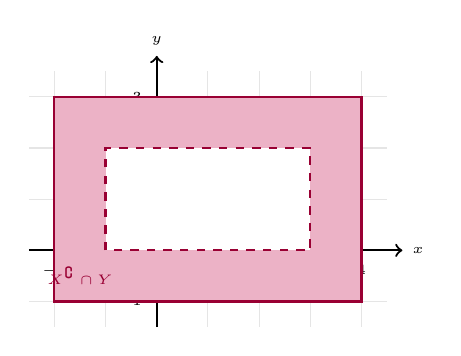
\begin{tikzpicture}[scale=0.65]
            % Grid & Axes
            \draw[gray!20, thin] (-2.5,-1.5) grid (4.5,3.5);
            \draw[->, thick] (-2.5,0) -- (4.8,0) node[right] {\tiny $x$};
            \draw[->, thick] (0,-1.5) -- (0,3.8) node[above] {\tiny $y$};
            
            % Ticks
            \foreach \x in {-2,-1,1,2,3,4} \draw (\x,0.1) -- (\x,-0.1) node[below] {\tiny $\x$};
            \foreach \y in {-1,1,2,3} \draw (0.1,\y) -- (-0.1,\y) node[left] {\tiny $\y$};
            
            % Full region [-2,4] x [-1,3] shaded
            \fill[purple!30] (-2,-1) rectangle (4,3);
            % Hole where X overlaps: [-1,3] x [0,2]
            \fill[white] (-1,0) rectangle (3,2);
            
            % Outer boundary of [-2,4] x [-1,3]
            \draw[thick, purple!80!black] (-2,-1) rectangle (4,3);
            % Boundary of the removed hole
            \draw[thick, dashed, purple!80!black] (-1,0) rectangle (3,2);
            
            \node[purple!80!black, font=\tiny] at (-1.5,-0.5) {$X^{\complement} \cap Y$};
        \end{tikzpicture}
        \caption{$X^{\complement}\cap([-2,4]\times[-1,3])$}
    \end{subfigure}

    \caption{Sketches for Exercise 6.4.}\label{fig:ex_6_4}
\end{figure}
\end{solution}

\begin{solution}\label{sol:6.5}\ref{ex:6.5}
    Ditto.
    \begin{figure}[htbp]
    \centering
    % Drawing 1: The set X (Annulus)
    \begin{subfigure}[b]{0.45\linewidth}
        \centering
        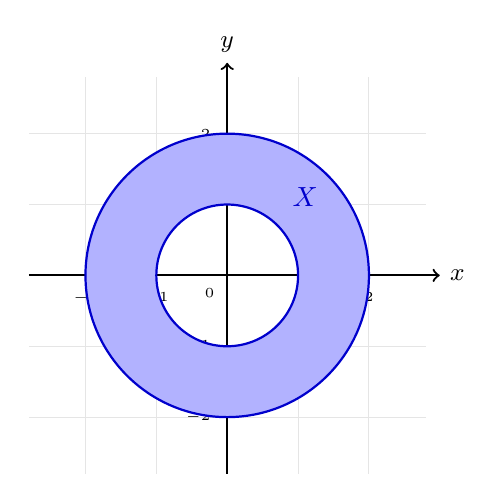
\begin{tikzpicture}[scale=0.9]
            % Grid & Axes
            \draw[gray!20, thin] (-2.8,-2.8) grid (2.8,2.8);
            \draw[->, thick] (-2.8,0) -- (3.0,0) node[right] {\small $x$};
            \draw[->, thick] (0,-2.8) -- (0,3.0) node[above] {\small $y$};
            
            % Ticks
            \foreach \x in {-2,-1,1,2} \draw (\x,0.1) -- (\x,-0.1) node[below] {\tiny $\x$};
            \foreach \y in {-2,-1,1,2} \draw (0.1,\y) -- (-0.1,\y) node[left] {\tiny $\y$};
            \node at (-0.25,-0.25) {\tiny $0$};

            % Shaded Annulus: Outer circle radius 2 minus inner circle radius 1
            \fill[blue!30, even odd rule] (0,0) circle (2cm) (0,0) circle (1cm);
            
            % Solid Boundaries
            \draw[thick, blue!80!black] (0,0) circle (2cm);
            \draw[thick, blue!80!black] (0,0) circle (1cm);
            
            \node[blue!80!black] at (1.1,1.1) {$X$};
        \end{tikzpicture}
        \caption{The set $X$ (Annulus $1 \le r \le 2$)}
    \end{subfigure}\qquad
    % Drawing 2: The Complement X^c
    \begin{subfigure}[b]{0.45\linewidth}
        \centering
        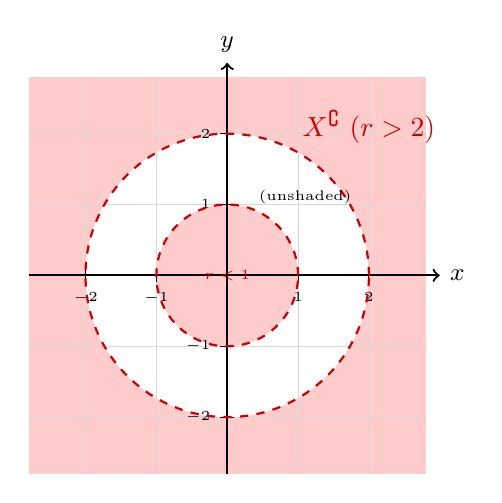
\begin{tikzpicture}[scale=0.9]
            % Outer bounding region shaded
            \fill[red!20] (-2.8,-2.8) rectangle (2.8,2.8);
            
            % Unshade the annulus X
            \fill[white] (0,0) circle (2cm);
            
            % Re-shade the inner core disk r < 1
            \fill[red!20] (0,0) circle (1cm);
            
            % Grid & Axes
            \draw[gray!30, thin] (-2.8,-2.8) grid (2.8,2.8);
            \draw[->, thick] (-2.8,0) -- (3.0,0) node[right] {\small $x$};
            \draw[->, thick] (0,-2.8) -- (0,3.0) node[above] {\small $y$};
            
            % Ticks
            \foreach \x in {-2,-1,1,2} \draw (\x,0.1) -- (\x,-0.1) node[below] {\tiny $\x$};
            \foreach \y in {-2,-1,1,2} \draw (0.1,\y) -- (-0.1,\y) node[left] {\tiny $\y$};
            
            % Dashed boundaries excluded from X^c
            \draw[thick, dashed, red!80!black] (0,0) circle (2cm);
            \draw[thick, dashed, red!80!black] (0,0) circle (1cm);
            
            \node[red!80!black] at (0,0) {\tiny $r < 1$};
            \node[red!80!black] at (2.0,2.1) {$X^{\complement}$ ($r > 2$)};
            \node at (1.1,1.1) {\tiny (unshaded)};
        \end{tikzpicture}
        \caption{The complement $X^{\complement}$ ($r < 1 \cup r > 2$)}
    \end{subfigure}

    \caption{Sketches for Exercise 6.5.}\label{fig:ex_6_5}
\end{figure}
\end{solution}

\begin{solution}\label{sol:6.6}\ref{ex:6.6}
    Ditto.
    
    \begin{figure}[htbp]
    \centering
    % Drawing 1: The set X (y < x^2)
    \begin{subfigure}[b]{0.45\linewidth}
        \centering
        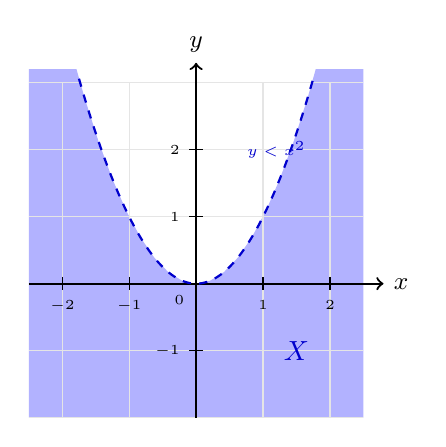
\begin{tikzpicture}[scale=0.85]
            % Bounding area for clip
            \begin{scope}
                \clip (-2.5,-2.0) rectangle (2.5,3.2);
                
                % Fill region below parabola y < x^2
                \fill[blue!30] plot[domain=-2.5:2.5, variable=\x] (\x, {\x*\x}) -- (2.5,-2.0) -- (-2.5,-2.0) -- cycle;
            \end{scope}

            % Grid & Axes
            \draw[gray!20, thin] (-2.5,-2.0) grid (2.5,3.0);
            \draw[->, thick] (-2.5,0) -- (2.8,0) node[right] {\small $x$};
            \draw[->, thick] (0,-2.0) -- (0,3.3) node[above] {\small $y$};
            
            % Ticks
            \foreach \x in {-2,-1,1,2} \draw (\x,0.1) -- (\x,-0.1) node[below] {\tiny $\x$};
            \foreach \y in {-1,1,2} \draw (0.1,\y) -- (-0.1,\y) node[left] {\tiny $\y$};
            \node at (-0.25,-0.25) {\tiny $0$};

            % Dashed parabola boundary y = x^2
            \draw[thick, dashed, blue!80!black, domain=-1.75:1.75, variable=\x, samples=100] plot (\x, {\x*\x});
            
            \node[blue!80!black] at (1.5,-1.0) {$X$};
            \node[blue!80!black, font=\tiny] at (1.2,2.0) {$y < x^2$};
        \end{tikzpicture}
        \caption{The set $X = \{(x,y) \in \mathbb{R}^2 : y < x^2\}$}
    \end{subfigure}\qquad
    % Drawing 2: The Complement X^c (y >= x^2)
    \begin{subfigure}[b]{0.45\linewidth}
        \centering
        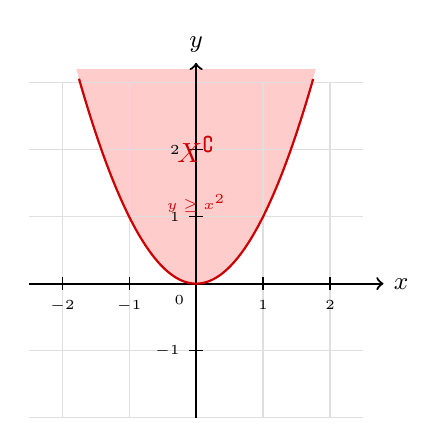
\begin{tikzpicture}[scale=0.85]
            % Bounding area for clip
            \begin{scope}
                \clip (-2.5,-2.0) rectangle (2.5,3.2);
                
                % Fill region on/above parabola y >= x^2
                \fill[red!20] plot[domain=-2.0:2.0, variable=\x] (\x, {\x*\x}) -- (2.5,3.5) -- (-2.5,3.5) -- cycle;
            \end{scope}

            % Grid & Axes
            \draw[gray!25, thin] (-2.5,-2.0) grid (2.5,3.0);
            \draw[->, thick] (-2.5,0) -- (2.8,0) node[right] {\small $x$};
            \draw[->, thick] (0,-2.0) -- (0,3.3) node[above] {\small $y$};
            
            % Ticks
            \foreach \x in {-2,-1,1,2} \draw (\x,0.1) -- (\x,-0.1) node[below] {\tiny $\x$};
            \foreach \y in {-1,1,2} \draw (0.1,\y) -- (-0.1,\y) node[left] {\tiny $\y$};
            \node at (-0.25,-0.25) {\tiny $0$};

            % Solid parabola boundary y = x^2
            \draw[thick, red!80!black, domain=-1.75:1.75, variable=\x, samples=100] plot (\x, {\x*\x});
            
            \node[red!80!black] at (0,2.0) {$X^{\complement}$};
            \node[red!80!black, font=\tiny] at (0,1.2) {$y \ge x^2$};
        \end{tikzpicture}
        \caption{The complement $X^{\complement} = \{(x,y) \in \mathbb{R}^2 : y \ge x^2\}$}
    \end{subfigure}

    \caption{Sketches for Exercise 6.6.}\label{fig:ex_6_6}
\end{figure}
\end{solution}
\section*{Solutions to Exercises from Section 7}

Skipped.


\section*{Solutions to Exercises from Section 8}

\begin{solution}\label{sol:8.1}\ref{ex:8.1}
    Let $A_{1}=\{ a,b,d,e,g,f \},A_{2}=\{ a,b,c,d \},A_{3}=\{ b,d,a \},A_{4}=\{ a,b,h \}$. Then,
    $$
    (1)~ \bigcup^{4}_{i=1}A_{i}= A_{1}\cup A_{2} \cup A_{3} \cup A_{4}=\{ a,b,c,d,e,f,g,h \}
    $$
    and 
    $$
    (2)~ \bigcap^{4}_{i=1}A_{i}=A_1 \cap A_2 \cap A_3 \cap A_4 =\{ a,b \}.
    $$
\end{solution}


\begin{solution}\label{sol:8.2}\ref{ex:8.2}
    Let $A_1= \{ 0,2,4,\dots,24 \},A_2=\{ 0,3,6,\dots,24 \},A_3=\{ 0,4,8,\dots,24 \}$. Then, 
    $$
    (1)~ \bigcup^{3}_{i=1}A_i=\{ 0,2,3,4,6,9,\dots,24 \}
    $$
    and 
    $$
    (2)~\bigcap^{3}_{i=1}A_i=\{ 0,12,14 \}.
    $$
\end{solution}


\begin{solution}\label{sol:8.3}\ref{ex:8.3}
    For each $n\in\N$, we let $A_n=\{ 0,1,2,3,4,\dots,n \}$. Let us first unpack what this means. Consider the following two interpretations: 
    $$
    A_0=\{ 0 \}, A_{1}=\{ 0,1 \},\dots \quad\quad A_1=\{ 0,1 \},A_2=\{ 0,1,2 \},\dots
    $$
    It is up to convention whether $\N=\{ 0,1,2,3,\dots \}$ or $\N=\{ 1,2,3,\dots \}$. Depending on the convention the answer might differ slightly. 
    Case $1$: 
    $$
    (1)~ \bigcup_{i\in\N}A_i= \N
    $$
    Case $2$: 
    $$
    (1)~ \bigcup_{i\in\N}A_i= \N\cup \{ 0 \}.
    $$
    Similarly for the second subpoint. 
    Case $1$: 
    $$
    (2)~ \bigcap_{i\in\N}A_i=\{ 0,1 \}
    $$
    and Case $2$:
    $$
    (2)~ \bigcap_{i\in\N}A_i=\{ 0 \}
    $$
\end{solution}

\begin{solution}\label{sol:8.4}\ref{ex:8.4}
    Let each $n\in \N$ with $A_{n} = \{ -2n, 0, 2n \}$, then similarly to before, we have 
    $$
    A_0 = \{ -2(0), 0, 2(0) \} \quad\quad A_1=\{ -2(1), 0, 2(1) \}, A_2=\{ -2(2), 0, 2(2) \}
    $$
    So, 
    $$
    \bigcup_{i\in\N}A_{i} = \{ \dots,-6,-4,-2,0,2,4,6,\dots \}
    $$
    and 
    $$
    \bigcap_{i\in\N}A_{i} = \{ 0 \}
    $$
    Similarly to before, if we assume that $\N=\N - \{ 0 \}$, then we will start from $A_1$ but this exercise will not be affected by that convetion like the previous one.
\end{solution}


\begin{solution}\label{sol:8.5}\ref{ex:8.5}
    
    $$
    (1)~ \bigcup_{i\in\N}[i,i+1]=[0,\infty)
    $$
    Here we assume that $0\in\N$, if you choose to assume the contrary, then the interval would start with $1$ instead of $0$.
    $$
    (2)~\bigcap_{i\in\N}[i,i+1]=\varnothing
    $$
    Since some pairs of intervals are disjoint ($[0,1]\cap[2,3]$). 
\end{solution}


\begin{solution}\label{sol:8.6}\ref{ex:8.6}
    $$
    (1)~\bigcup_{i\in\N}[0,i+1]=[0,\infty)
    $$
    and 
    $$
    (2)~\bigcap_{i\in\N}[0,i+1]=[0,1] \text{ or } [0,2] \text{ depending on whether we include } 0\in\N
    $$
\end{solution}


\begin{solution}\label{sol:8.7}\ref{ex:8.7}
    
    $$
    (1)~\bigcup_{i\in\N}\R\times[i,i+1]=\R\times [0,\infty)
    $$
    Again, in the above, convention matters, it will be the differnece between $[1,\infty)$ and the answer provided above. 
    $$
    (2)~\bigcap_{i\in\N}\R\times[i,i+1]=\varnothing
    $$
\end{solution}


\begin{solution}\label{sol:8.8}\ref{ex:8.8}
    
    $$
    (1)~\bigcup_{a\in\R}\{ a \}\times[0,1]=\R \times [0,1]
    $$
    We know that $a\in\R$ means that $a$ is any real number such that $\sqrt2\times[0,1]$ for example. 
    $$
    (2)~\bigcap_{a\in\R}\{ a \}\times[0,1]=\varnothing
    $$
\end{solution}


\begin{solution}\label{sol:8.9}\ref{ex:8.9}
    
    $$
    (1)~\bigcup_{X\in\powerset(\N)}X=\N
    $$
    The way to think about it is that because $X\in\powerset(\N)$, then $X$ can be any subset of the natural numbers. The union of those subsets would be the natural numbers. 
    $$
    (2)~\bigcap_{X\in\powerset(\N)}X=\varnothing
    $$
    Important here is to remember that the empty set is part of $\powerset(\N)$.
\end{solution}

\begin{solution}\label{sol:8.10}\ref{ex:8.10}
    
    $$
    (1)~\bigcup_{x\in[0,1]}[x,1]\times[0,x^{2}]=\{ (u,v):0\le u\le 1, 0\le v \le u^{2} \}
    $$
    and 
    $$
    (2)~\bigcap_{x\in[0,1]}[x,1]\times[0,x^{2}]=\{ (1,0) \}
    $$
\end{solution}


\begin{solution}\label{sol:8.11}\ref{ex:8.11}
    Yes, this is always true. Informally speaking, the intersection of two sets is almost always smaller than their union. Consider the example: 
    $$
    \{ 1,2,3 \}\cup \{ 2,3,4 \}= \{ 1,2,3,4 \} \quad\quad \{ 1,2,3 \}\cap \{ 2,3,4 \}=\{ 2,3 \}.
    $$
    In the case when the intersection is empty and the two sets disjoint, then we know that the empty set is a subset of any set, so the statement still holds. 

    For a more formal proof, let $\alpha\in I$, then suppose for some $x\in\alpha_{0}$. Since, $x\in\alpha_{0}$ and $\alpha\in I$, then $x\in A_{\alpha_{0}}$. Therefore, $x\in\bigcup_{\alpha\in I}A_{\alpha}$.
\end{solution}

\begin{solution}\label{sol:8.12}\ref{ex:8.12}
    Now we consider the relationship between $\bigcap_{\alpha\in I}A_{\alpha}=\bigcup_{\alpha\in I}A_{\alpha}$. Clearly if they are equal the first thing to consider would be that two sets are equal, meaning 
    $$
    \{ 1,2,3 \}\cap \{ 1,2,3 \}=\{ 1,2,3 \} \quad\quad \{ 1,2,3 \}\cup \{ 1,2,3 \}=\{ 1,2,3 \}
    $$
    In other words, that all $A_{\alpha}$ are equal. 
\end{solution}

\begin{solution}\label{sol:8.13}\ref{ex:8.13}
    If $J\ne\varnothing, J\subseteq I$, then is it true that $\bigcup_{\alpha\in J}A_{\alpha}\subseteq \bigcup_{\alpha\in I}A_{\alpha}$? Let us break down the statement. First, suppose that $J=\{ 1,2,3 \}$ and $I=\{ 1,2,3,4 \}$, then the statement would be true. Intuitively, the idea is that $J$ can be at most as large as $I$. If we think about the definition of big union 
    $$
    \bigcup_{\alpha\in J}A_\alpha=\{ x: \exists \alpha \in I, x\in A_\alpha \},
    $$
    so, the requirement is that at \emph{at least one} $x$ that is a member of $A_{\alpha}$, then since $J\subseteq I$, it follows by definition of subsets that the equivalence holds. 
    
    Now, let's consider the second one. The definition of big intersection is $\forall \alpha \in I, x\in A_{\alpha}$ to be true. This however is not necessitated by the definition of subets. So it could be true, but it \emph{does not} hold in general. 
\end{solution}

\begin{solution}\label{sol:8.14}\ref{ex:8.14}
    If $J\ne\varnothing,J\subseteq I$, then $\bigcap_{\alpha\in I}A_{\alpha}\subseteq \bigcap_{\alpha \in J}A_{\alpha}$. Now, let some arbitrary element $x\in \bigcap_{\alpha\in I}A_{\alpha}$, then $\forall \alpha \in I, x\in A_{\alpha}$. Similar to before, if $J\subseteq I$, then $J$ is at most as big as $I$. Since, all $x\in A_{\alpha}$ for an arbitrary $x$, then it follows that $\forall \alpha \in J, x \in A_{\alpha}$. Thus, $x\in\bigcap_{\alpha\in J}A_{\alpha}$.
\end{solution}

\section{Solutions to Exercises From Section 11}
\begin{solution}\label{sol:2.11}\ref{ex:2.11}
    \begin{enumerate}
        \item This is a false statement. 
        \item This is a true statement. 
        \item This is a true statement. 
        \item This is not a statement. 
        \item This is a true statement. 
        \item This is a true statement. 
        \item This is a false statement. 
        \item This is a false statement. 
        \item This is an open sentence/formula. 
        \item This is a true statement. 
        \item This is an open sentence/formula. 
        \item This is a true statement. It is called a \emph{tautology}.
        \item This is a true statement. 
        \item This is not a statement. 
        \item This is technically a statement since it can be either true or false. But its truth value is unclear. It is similar to a conjecture. 
    \end{enumerate}
\end{solution}

\section*{Solutions to Exercises From Section 12}
\begin{solution}\label{sol:2.12}\ref{ex:2.12}
    \begin{enumerate}
        \item $P$: `The number $8$ is even', $Q$: `The number $8$ is a power of $2$', so $P\land Q$. 
        \item $P$: The matrix $A$ is invertible. Then $\neg P$. 
        \item $x\ne y$ is the same as $\neg(x=y)$, so if $P:x=y$, then $\neg P:x\ne y$. 
        \item $x < y$ is the same as $\ne(x\ge y)$, so similarly to above we have $\neg P$, where $P$ is $x\ge y$. 
        \item $y\ge x$ is equivalent to $\neg(y<x)$, so again we can simply state $\neg P$, where $P$ is $y<x$. 
        \item $P$: Scheduled for Wednesday, $Q$: Scheduled for Friday, so $P\lor Q$.\footnote{When we later look at quantifiers and predicates, we will find that there is another more expressive way to represent the above statement: $\exists x(P(x)\lor Q(x))$ where $x$ represents the quiz. Furthermore, we can say that there is a quiz on Wednesday or Friday but not both days: $\exists x((P(x)\lor Q(x))\land \neg(P(x)\land Q(x)))$.}
        \item $P:x=0$ and $Q:y=0$ so, $P\land\neg Q$. 
        \item $P:x=0$ and $Q:y=0$, so $P\lor Q$. Similarly, to the footnote, we can transform this accordingly with predicates and quantifiers. 
        \item $x\in A\land x\notin B$.
        \item $x\in A\lor x\in B$.
        \item This one is slightly trickier. Let $A$ be a member of the set, then $A\in\powerset(\N)$, so now we have to `append' the condition on $A$, which is $\lvert A^{\complement} \rvert<\infty$, so together we have $A\in\powerset(\N)\land \lvert A^{\complement} \rvert<\infty$.
        \item $H$: Happy families, $A$: Alike, $W$: Unhappy in its own way. Breaking down the statement we have, if a family is happy, then it is alike, \emph{and} if it is not happy, then it is unhappy in its own way. Therefore, $(H\Rightarrow A)\land(\neg H\Rightarrow W)$. If we don't want to use arrows or conditional statements, the formula looks thus: $(\neg H\lor A)\land (H\lor W)$.
        \item $H$: Human beings want to be good, $S$: Too good, $R$: All the time. So, $H\land \neg S \land \neg R$. 
        \item $P$: A man should look for what is, $Q$: A man should look for what he think should be. Then, $P\land \neg Q$.
    \end{enumerate}
\end{solution}
\section{Solutions for Exercises from Section 13}
\begin{solution}\label{sol:2.13}\ref{ex:2.13}
    \begin{enumerate}
        \item If the determinant is not zero, then the matrix is invertible. 
        \item If a function is differentiable, then it is continuous. 
        \item If a function is continuous, then it is integrable. 
        \item If a function is a polynomial, then it is rational. 
        \item If an integer is divisible by $8$, then it is divisible by $4$. 
        \item If a surface has only one side, then it is non-orientable. 
        \item If a series converges absolutely, then it converges. 
        \item If the ratio $r$ of a geometric series is $\lvert r \rvert<1$, then the series converges. 
        \item If a function is continuous, then the function is also integrable. 
        \item If the descriminant is negative, then the quadratic equation has no real solutions. 
        \item If you stop writing, you fail. 
        \item In general, if people accept facts as truth, then the facts agree with what they already believe. 
        \item If people agree with me, then I feel I must be wrong. 
    \end{enumerate}
\end{solution}




\end{document}